\setchapterpreamble[u]{\margintoc}
\chapter{Linguaggi liberi dal contesto}\label{cha:CFG}
\labch{Linguaggi liberi dal contesto}







\section{Grammatiche Context-Free}\label{sec:CFG}

\begin{example}
	Sia $G=(V,T,O,E)$, con $V=\{E,I\}$ e $T=\{a,b,0,1,(,),+,*\}$
	quindi ho le seguenti regole, è di tipo 3:
	\begin{enumerate}
		\item $E\to I$
		\item $E\to E+E$
		\item $E\to E*E$
		\item $E\to (E)$
		\item $I\to a$
		\item $I\to b$
		\item $I\to Ia$
		\item $I\to Ib$
		\item $I\to I0$
		\item $I\to I1$
	\end{enumerate}
	voglio ottenere $a*(a+b00)$
	sostituisco sempre a destra (right most derivation)
	$$E\to E*E\to E*(E)\to E*(E+E)\to E*(E+I)\to E+(E+I0)$$
	$$\to R+(I+b00)\to E*(a+b00)\to I*(a+b00)\to a*(a+b00)$$

	usiamo ora \textit{l'inferenza ricorsiva}:
	\begin{center}
		\begin{tabular}{|c|c|c|c|c|}
			\hline
			passo & stringa ricorsiva & var & prod & passo stringa impiegata \\
			1     & a                 & I   & 5    & $\backslash$            \\
			\hline
			2     & b                 & I   & 6    & $\backslash$            \\
			\hline
			3     & b0                & I   & 9    & 2                       \\
			\hline
			4     & b00               & I   & 9    & 3                       \\
			\hline
			5     & a                 & E   & 1    & 1                       \\
			\hline
			6     & b00               & E   & 1    & 4                       \\
			\hline
			7     & a+b00             & E   & 2    & 5,6                     \\
			\hline
			8     & (a+b00)           & E   & 4    & 7                       \\
			\hline
			9     & a*(a+b00)         & E   & 3    & 5, 8                    \\
			\hline
		\end{tabular}
	\end{center}
\end{example}
definisco formalmente la derivazione $\to$:
\begin{definition}
	Prendo una grammatica $G=(V,T,P,S)$, grammatica CFG. Se $\alpha A \beta$ è una stringa tale che $\alpha,\beta\in (V\cup T)^*$, appartiene sia a variabili che terminali. Sia $A\in V$ e sia $a\to \gamma$ una produzione di $G$. Allora
	scriviamo:
	$$\alpha A \beta \to \alpha\gamma\beta$$
	con $\gamma\in (V\cup T)^*$.\\
	Le sostituzioni si fanno indipendentemente da $\alpha$ e $\beta$.
	Questa è quindi la definizione di derivazione.
\end{definition}
\begin{definition}
	Definisco il simbolo $\to _*$, ovvero il simbolo di \textit{derivazioni in 0 o più passi}. Può essere definito in modo ricorsivo. Per induzione sul numero di passi.
	\begin{itemize}
		\item la base dice che  $\forall \alpha\in (V\cup T)^*,\, \alpha\to * \,\alpha$
		\item il passo è: se $\alpha\to_{G_*} \,\beta $ e $ \beta \to_{G_*} \,\gamma$ allora $\alpha\to_* \,\gamma$
	\end{itemize}
	Si può anche dire che $\alpha\to_{G_*}\, \beta$ sse esiste una sequenza di stringhe $\gamma_1,...,\gamma_n$ con $n\geq 1$ tale che $\alpha=\gamma_1$, $\beta=\gamma_n$ e $\forall i,\, 1<i<n-1$ si ha che $\gamma_1\to \gamma_{i+1}$
	la derivazione in 0 o più passi è la chiusura transitiva della derivazione
\end{definition}
\begin{definition}
	avendo ora definito questi simboli possiamo definire una forma sentenziale. Infatti è una stringa $\alpha$ tale che:
	$$\forall \alpha\in (V\cup T)^* \mbox{ tale che }S\to_{G_*}\, \alpha$$
\end{definition}
\begin{definition}
	data $G=(V,T,P,S)$ si ha che $L(G)=\{w\in T^* |\, S\to_{G_*}\, w\}$ ovvero composto da stringhe terminali che sono derivabili o 0 o più passi.
\end{definition}
\begin{example}
	formare una grammatica CFG per il linguaggio:
	$$L=\{0^n 1^n| n\geq 1\}=\{01, 0011, 000111,...\}$$
	con $x^n$ intendo una concatenazione di $n$ volte $x$ (che nel nostro caso sono 0 e 1).\\
	posso scrivere:
	$$0^n 1^n =00^{n-1} 1^{n-1}1$$
	il nostro caso base sarà la stringa $01$, Poi si ha:
	$G=(V,T,P,S)$, $T=\{0,1\}$, $V=\{S\}$, il caso base $S\to 01$  e $S\to 0S1$
	il caso passo è quindi: se $w= 0^{n-1}1^{n-1}\in L$ allora $0w1\in L$.\\
	Ora voglio dimostare che $000111\in L$, ovvero $S\to*\, 000111$:\\
	$$S\to\, 0S1 \to 00S11\to 000S111$$
\end{example}
\begin{theorem}
	data la grammatica $G=\{V,T,P,S)$ CFG e $\alpha\in (V\cup T)^*$. Si ha che vale $S\to_*\, \alpha$ sse $S\to_{lm_*}\, \alpha$ sse $S\to_{rm_*}\, \alpha$. Con $\to_{lm_*}$ simbolo di \textit{left most derivation }e $\to_{rm_*}$ simbolo di \textit{right most derivation}
\end{theorem}
\begin{example}
	formare una grammatica CFG per il linguaggio:
	$$L=\{0^n 1^n| n\geq 0\}=\{\varepsilon, 01, 0011, 000111,...\}$$
	stavolta abbiamo anche la stringa vuota. Il caso base stavolta è $S\to\varepsilon| \, 0S1$
\end{example}
\begin{example}
	Fornisco una CFG per $L=\{a^n|n\geq 1\}=\{a, aa, aaa,...\}$.
	La base è $a$ \\il passo è che se $a^{n-1}\in L$ allora $a^{n-1}a\in L$ ( o che $aa^{n-1}\in L$).\\
	Si ha la grammatica $G=\{V,T,P,S)$, $V=\{S\}$, $T=\{a\}$ e si hanno $S\to a|\,Sa$ (o  $S\to a|\,aS$). Dimostro che $a^3\in L$.
	$$S\to Sa \to Saa\to aaa$$
	oppure
	$$S\to aS\to aaS\to aaa$$
\end{example}
\begin{example}
	trovo una CFG per $L=\{(ab)^n|n\geq 1\}=\{ab, abab, ababab,...\}$\\
	La base è $ab$ \\il passo è che se $(ab)^{n-1}\in L$ allora $(ab)^{n-1}ab\in L$.\\
	Si ha la grammatica $G=\{V,T,P,S)$, $V=\{S\}$, $T=\{a,b\}$ (anche se in realtà $T=\{ab\}$) e si hanno $S\to ab|\,Aab$. Poi dimostro come l'esempio sopra
\end{example}
\begin{example}
	trovo una CFG per $L=\{a^n c b^n|n\geq 1\}=acb,aacbb,aaacbbb,...\}$\\
	Il caso base è $acb$ il passo è che se $a^{n-1}cb^{n-1}\in L$ allora $a^{n-1}cb^{n-1}acb\in L$
	Si ha la grammatica $G=\{V,T,P,S)$, $V=\{S\}$, $T=\{a,b,c\}$ e si hanno $S\to aSb|acb$.\\
	dimostro che $aaaacbbbbb\in L$:
	$$S\to aSb\to aaSbb\to aaaaSbbb\to aaaacbbbb$$

	provo a usare anche una grammatica regolare, con le regole $S\to aS|c$, $c\to cB$ e $B\to bB|b$;
	$$S\to aS\to aaS\to aaC\to aacB\to aacb...$$
	non si può dimostrare in quanto non si può imporre una regola adatta
\end{example}
\begin{example}
	$L=\{a^n c b^{n-1}|n\geq 2\}$, con $a^n c b^{n-1}=a^{n-1}acb^{n-1}$. $S\to aSb|aacb$. Quindi:
	$$S\to aSb\to aaaccbb\in L$$
\end{example}
\begin{example}
	cerco CFG per $L=\{a^n c^k b^n|\,n,\,k>0\}$. $a$ e $b$ devono essere uguali, uso quindi una grammatica context free, mentre $c$ genera un linguaggio regolare.\\
	Si ha la grammatica $G=\{V,T,P,S)$, $V=\{S,C\}$, $T=\{a,b,c\}$ e si hanno $S\to aSb|aCb$ e $C\to cC|c$. dimostro che $aaaccbbb\in L, n=3,\, k=2$:
	$$S\to aSb \to aaSbb\to aaaCbbb\to aaacCbbb\to aaaccbbb$$
\end{example}
\begin{example}
	scrivere CFG per $L=\{a^nb^nc^kb^k|\, n,\,k\geq 0\}
	$
	$$=\{w\in\{a,b,c,d\}^*|\,a^nb^nc^kb^k|\, n,\,k\geq 0\}$$
	quindi L concatena due linguaggi $L1$ e $L2$, $X=\{a^nb^n\}$ e $Y=\{c^kd^k\}$:
	$$X\to aXb | \varepsilon$$
	$$Y\to cYd | \varepsilon$$
	$$S\to XY$$
	voglio derivare $abcd$:
	$$S\to XY \to XcYd\to aXbcYd\to aXbc\varepsilon d\to a\varepsilon bc\varepsilon d\to abcd$$
	voglio derivare $cd$
	$$S\to XY\to Y\to cYd\to cd$$
\end{example}
Quindi se ho $w\in L1, L2$, ovvero appartenente ad una concatenazione di linguaggi prima uso le regole di un linguaggio, poi dell'altro e infine ottengo il risultato finale.\\
\begin{example}
	scrivere CFG per $L=\{a^nb^kc^kd^n|\, n>0,\, k\geq 0\}
	$.
	$$S\to aSd|\, aXd$$
	$$X\to bXc| \varepsilon$$
	derivo $aabcdd$:
	$$S\to aSd\to aaXdd\to aabXcdd\to aabcdd$$
\end{example}
\begin{example}
	scrivere CFG per $L=\{a^ncb^nc^mad^m|\, n>0,\, m\geq 1\}
	$.
	$$S\to XY$$
	$$X\to aXb|c$$
	$$Y\to cUd| cad$$
	$$S\to XY\to cY\to ccad$$
\end{example}
\begin{example}
	scrivere CFG per $L=\{a^{n+m}xc^nyd^m|\, n,\, m\geq 0\}
	$. $a^{n+m}=a^na^m \mbox{ o } a^ma^n$. Si hanno 2 casi:
	\begin{enumerate}
		\item $L=\{a^na^m xc^nyd^m|\, n,\, m\geq 0\}
					$
		\item $L=\{a^ma^n xc^nyd^m|\, n,\, m\geq 0\}
					$
	\end{enumerate}
	ma solo  $L=\{a^ma^n xc^nyd^m|\, n,\, m\geq 0\}
	$ può generare una CFG (dove non si possono fare incroci, solo concatenazioni e inclusioni/innesti).
	$$S\to aSd| Y$$
	$$Y\to Xy$$
	$$X\to aXc|x$$
	si può fare in 2:
	$$S\to aSd| Xy$$
	$$X\to aXc|x$$
	derivo con $m=n=1$, $aaxcyd$:
	$$S\to aSd\to aXyd\to aaXcyd\to aaxcyd$$
\end{example}
\begin{example}
	scrivere CFG per $L=\{a^nb^m|\, n\geq m \geq 0\}
	$.$$L=\{\varepsilon, a, ab, aa, aab, aabb, aaa, aaab, aaabb, aaabbb,...\}$$
	Se $n\geq m$ allora $\exists k\geq 0 \to n=m+k$. Quindi:
	$$l=\{a^{m+k}b^m|m,k\geq0\}$$ si può scrivere in 2 modi:
	\begin{enumerate}
		\item $l=\{a^ma^kb^m|m,k\geq0\}$ quindi con innesto
		\item $l=\{a^ka^mb^m|m,k\geq0\}$quindi con concatenazione
	\end{enumerate}
	entrambi possibili per una CFG:
	\begin{enumerate}
		\item
					$$S\to XY$$
					$$X\to aX|\varepsilon \mbox{ si può anche scrivere } X\to Xa|\varepsilon$$
					$$Y\to aYb|\varepsilon$$
					oppure
					$$S\to aS|X$$
					$$X\to aXb| \varepsilon$$
		\item
					$$S\to aSb|\varepsilon$$
					$$X\to aX|\varepsilon$$
	\end{enumerate}
\end{example}
\begin{example}
	scrivere CFG per $L=\{a^nb^{m+n}c^h|\, m>h\geq0,\, n\geq0\}
	$.\\
	Se $n>h$ allora $\exists k \to n= h+k$, quindi:
	$$L=\{a^nb^{m+h+k}c^h|\, m>h\geq0,\, n\geq0\}$$. ovvero:
	$$L=\{a^nb^nb^kb^hc^h|\, m\geq 0, k>0, h\geq 0\}$$
	si ha:
	$$S\to XYZ$$
	$$X\to aXb|\varepsilon$$
	$$Y\to Yb|b$$
	$$Z\to bZc|\varepsilon$$
	si può anche fare:
	$$S\to XY$$
	$$X\to aXb|\varepsilon$$
	$$Y\to bYc|Z$$
	$$Z\to bZ|b$$
\end{example}
\begin{example}
	scrivere CFG per $L=\{a^nb^mc^k|\, k>n+m,\, n,m\geq 0\}
	$.\\
	per $n=m=0,\, k=1$ avrò la stringa $c$.
	se $k>n+m$ allora $\exists l>0\to k=n+m+l$ quindi:
	$$L=\{a^nb^mc^{n+m+l}|\, l>0,\, n,m\geq 0\}
	$$
	$$=L=\{a^nb^mc^nc^mc^l|\, l>0,\, n,m\geq 0\}$$
	sistemando:
	$$=L=\{a^nb^mc^lc^mcnl|\, l>0,\, n,m\geq 0\}$$
	quindi:
	$$S\to aSc|X$$
	$$X\to bXc|Y$$
	$$Y\to cY|c$$
\end{example}
\newpage
\begin{example}
	scrivere CFG per $L=\{a^nxc^{n+m}y^hz^kd^{m+h}|\, n,m,k,h\geq 0\}
	$.\\
	ovvero:
	$$L=\{a^nxc^nc^my^hz^kd^hd^m|\, n,m,k,h\geq 0\}$$
	quindi avrò:
	$$S\to XY$$
	$$X\to aXc|x$$
	$$Y\to cYd|W$$
	$$W\to yWd|X$$
	$$Z\to zZ|\varepsilon$$
\end{example}
\begin{example}
	vediamo un esempio di grammatica dipendente dal contesto:
	$$L=\{a^nb^nc^n|\, n\geq 1\}$$
	$G=\{V,T,P,S\}=\{(S,B,C,X)\}=\{(a,b,c),P,S\}$
	ecco le regole di produzione (qui posso scambiare variabili a differenza delle context free):
	\begin{enumerate}
		\item $S\to aSBC$
		\item $S\to aBC$
		\item $CB\to XB$
		\item $XB\to XC$
		\item $XC\to BC$
		\item $aB\to ab$
		\item $bB\to bb$
		\item $bC\to bc$
		\item $cC\to cc$
	\end{enumerate}
	vediamo un esempio di derivazione:
	per $n=1$ ho $abc$ ovvero:
	$$S\to aBC\to abC\to abc$$
	con $n=2$ ho $aabbcc$:
	$S\to aSBC\to aaBCBC\to aaBXBC\to aaBXCC\to aaBBCC\to aabBCC\to aabbCC\to aabbcC\to aabbcc$\\
	%vedere dimostrazione pag 14 soligo
\end{example}
\newpage
\begin{example}
	vediamo un esempio di grammatica dipendente dal contesto:
	$$L=\{a^nb^mc^nd^m|\, n,m\geq 1\}$$
	Si ha:
	$$G=(\{S,X,C,D,Z\},\{a,b,c,d\},P,S)$$
	con le seguenti regole di produzione:
	\begin{itemize}
		\item $S\to aSc|\, aXc$
		\item $X\to bXD|\, bD$
		\item $DC\to CD$
		\item $DC\to DZ$
		\item $DZ\to CZ$
		\item $XZ\to CD$
		\item $bC\to bc$
		\item $cC\to cc$
		\item $cD\to cd$
		\item $dD\to dd$
	\end{itemize}
	provo a derivare $aabbbccddd$ quindi con $n=2,\,m=3$:\\
	$$S\to aSC\to aaXCC\to aabXDCC\to aabbXDDCC\to $$
	$$aabbbDDDCC\to aabbbCCDDD\to aabbbccddd$$
\end{example}
\begin{example}
	Sia $L=\{w\in\{a,b\}^*|\, \mbox{ w contiene lo stesso numero di a e b}\}$:
	$$S\to aSbS|\,bSaS|\, \varepsilon$$
	dimostro per induzione che è corretto:
	\begin{itemize}
		\item \textbf{caso base:} $|w|=0\to w=\varepsilon$
		\item \textbf{caso passo:} si supponga che $G$ produca tutte le stringhe (di lunghezza $<$ di $n$) di $\{a,b\}^*$ con lo stesso numero di \textit{a} e \textit{b} e dimostro che produce anche quelle di lunghezza $n$, sia:
					$$w\in \{a,b\}^* \mid\, |w|=n \mbox{ con\textit{ a} e \textit{b} in egual numero, }m(a)=m(b) \mbox{ con m() che indica il numero di caratteri}$$
					quindi si ha che:
					$$w=aw_1bw_2\mbox{ o } w=bw_1aw_2$$
					sia.
					$$k_1=m(a)\in w_1=m(b)\in w_1$$
					$$k_2=m(a)\in w_2=m(b)\in w_2$$
					allora:
					$$k_1+k_2+1=m(a)\in w= m(b)\in W$$
					sapendo che $|w_1|<n$ e $|w_2|<n$ allora $w_1$ e $w_2$ sono egnerati da G per ipotesi induttiva
	\end{itemize}
\end{example}

\section{Alberi Sintatici}
\begin{definition}
	Data una grammatica CFG, $G=\{V,T,P,S\}$ un \textbf{albero sintattico} per $G$ soddisfa le seguenti condizioni:
	\begin{itemize}
		\item ogni nodo interno è etichettato con una variabile in $V$
		\item ogni foglia è anch'essa etichettata con una variabile o col simbolo di terminale T o con la stringa vuota $\varepsilon$ (in questo caso la foglia è l'unico figlio del padre)
		\item se un nodo interno è etichettato con A i suoi figli saranno etichettati con X1, ..., Xk e $A\to  X1, ..., Xk$ sarà una produzione di $G$ in $P$. Se un $X_i$ è $\varepsilon$ sarà l'unica figlio e $A\to \varepsilon$ sarà comunque una produzione di $G$
	\end{itemize}
	La concatenazione in ordine delle foglie viene detto \textbf{prodotto dell'albero}
\end{definition}
\newpage
\begin{example}
	Usiamo l'esempio delle stringhe palindrome:
	$$P\to 0P0|\,1P1|\varepsilon$$
	sia il seguente albero sintatico:
	\begin{center}
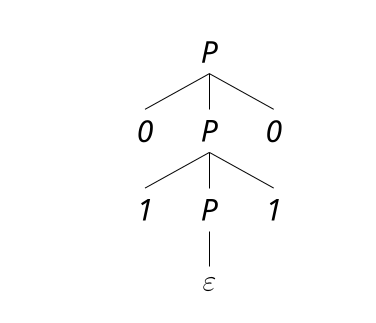
\includegraphics{example_1.1.1.png
}
%		\psframebox[linestyle=none,framesep=10pt]{%
%			\pstree{\LFTw{t}{\fontspec{Noto Sans}[Script=Latin]P}}{\pstree{\Tp[edge=none]}{%
%					\LFTw{t}{\fontspec{Noto Sans}[Script=Latin]0}
%					\pstree{\LFTw{t}{\fontspec{Noto Sans}[Script=Latin]P}}{\pstree{\Tp[edge=none]}{%
%							\LFTw{t}{\fontspec{Noto Sans}[Script=Latin]1}
%							\pstree{\LFTw{t}{\fontspec{Noto Sans}[Script=Latin]P}}{\pstree{\Tp[edge=none]}{%
%									\LFTw{t}{\fontspec{Noto Sans}[Script=Latin]$\varepsilon$}}}
%							\LFTw{t}{\fontspec{Noto Sans}[Script=Latin]1}}}
%					\LFTw{t}{\fontspec{Noto Sans}[Script=Latin]0}}}}
	\end{center}
\end{example}
\begin{example}
	Si ha:
	$$E\to I|\, E+E|\, E*E|\, (E)$$
	$$I\to a|\,b|\,Ia|\,Ib|\,I0|\,I1$$
	un albero sintattico per $a*(a+b00)$ può essere:
	\begin{center}
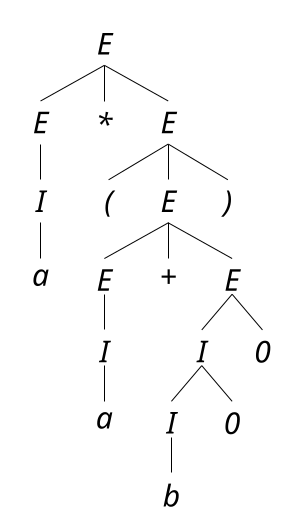
\includegraphics{example_1.1.2.png}
%		\psframebox[linestyle=none,framesep=10pt]{%
%			\pstree{\LFTw{t}{\fontspec{Noto Sans}[Script=Latin]E}}{\pstree{\Tp[edge=none]}{%
%					\pstree{\LFTw{t}{\fontspec{Noto Sans}[Script=Latin]E}}{\pstree{\Tp[edge=none]}{%
%							\pstree{\LFTw{t}{\fontspec{Noto Sans}[Script=Latin]I}}{\pstree{\Tp[edge=none]}{%
%									\LFTw{t}{\fontspec{Noto Sans}[Script=Latin]a}}}}}
%					\LFTw{t}{\fontspec{Noto Sans}[Script=Latin]*}
%					\pstree{\LFTw{t}{\fontspec{Noto Sans}[Script=Latin]E}}{\pstree{\Tp[edge=none]}{%
%							\LFTw{t}{\fontspec{Noto Sans}[Script=Latin](}
%								\pstree{\LFTw{t}{\fontspec{Noto Sans}[Script=Latin]E}}{\pstree{\Tp[edge=none]}{%
%										\pstree{\LFTw{t}{\fontspec{Noto Sans}[Script=Latin]E}}{\pstree{\Tp[edge=none]}{%
%												\pstree{\LFTw{t}{\fontspec{Noto Sans}[Script=Latin]I}}{\pstree{\Tp[edge=none]}{%
%														\LFTw{t}{\fontspec{Noto Sans}[Script=Latin]a}}}}}
%										\LFTw{t}{\fontspec{Noto Sans}[Script=Latin]+}
%										\pstree{\LFTw{t}{\fontspec{Noto Sans}[Script=Latin]E}}{\pstree{\Tp[edge=none]}{%
%												\pstree{\LFTw{t}{\fontspec{Noto Sans}[Script=Latin]I}}{\pstree{\Tp[edge=none]}{%
%														\pstree{\LFTw{t}{\fontspec{Noto Sans}[Script=Latin]I}}{\pstree{\Tp[edge=none]}{%
%																\LFTw{t}{\fontspec{Noto Sans}[Script=Latin]b}}}
%														\LFTw{t}{\fontspec{Noto Sans}[Script=Latin]0}}}
%												\LFTw{t}{\fontspec{Noto Sans}[Script=Latin]0}}}}}
%								\LFTw{t}{\fontspec{Noto Sans}[Script=Latin])}}}}}}
	\end{center}
\end{example}
\newpage
Data una CFG si ha che i seguenti cinque enunciati si equivalgono:
\begin{enumerate}
	\item la procedura di inferenza ricorsiva stailisce che una stringa $w$ di simboli terminali appartiene al linguaggio $L(A)$ con $A$ variabile
	\item $A\to ^*w$
	\item $A\to^*_{lm}w$
	\item $A\to^*_{rm}w$
	\item esiste un albero sintattico con radice $A$ e prodotto $w$
\end{enumerate}
queste 5 proposizioni si implicano l'uni l'altra:
\begin{center}
	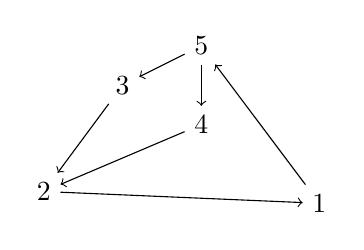
\begin{tikzpicture}
		\node (top) at (0,0) {5};
		\node (a) at(-1,-0.5) {3};
		\node (b) at(0,-1) {4};
		\node (c) at(-2.0,-1.85) {2};
		\node (d) at(1.5,-2) {1};
		\draw [->] (top) -- (a);
		\draw [->] (top) -- (b);
		\draw [->] (a) -- (c);
		\draw [->] (b) -- (c);
		\draw [->] (c) -- (d);
		\draw [->] (d) -- (top);
	\end{tikzpicture}
\end{center}
vediamo qualche dimostrazione di implicazione tra queste proposizioni:
\begin{proof}[da 1 a 5]
	si procede per induzione:
	\begin{itemize}
		\item \textbf{caso base:} ho un livello solo (una sola riga), $\exists A\to w$:
					$$\overset{A}{\overset{\triangle}w}$$
		\item \textbf{caso passo:} suppongo vero per un numero di righe $\leq n$, lo dimsotro per $n+1$ righe:
					$$A\to X_1,X_2,...,X_k$$
					$$w=w_1,w_2,...,w_k$$
					ovvero, in meno di $n+1$ livelli:
					\begin{center}
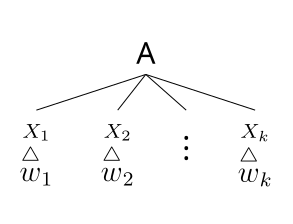
\includegraphics{caso_passo.png}
					% \psframebox[linestyle=none,framesep=10pt]{%
%				      \pstree{\LFTw{t}{\fontspec{Noto Sans}[Script=Latin]A}}{\pstree{\Tp[edge=none]}{%
%						      \LFTw{t}{\fontspec{Noto Sans}[Script=Latin]$\overset{X_1}{\overset{\triangle}w_1}$}
%						      \LFTw{t}{\fontspec{Noto Sans}[Script=Latin]$\overset{X_2}{\overset{\triangle}w_2}$}
%						      \LFTw{t}{\fontspec{Noto Sans}[Script=Latin]$\vdots$}
%						      \LFTw{t}{\fontspec{Noto Sans}[Script=Latin]$\overset{X_k}{\overset{\triangle}w_k}$}}}}
					\end{center}
	\end{itemize}
\end{proof}
\begin{proof}[da 5 a 3]
	procedo per induzione:
	\begin{itemize}
		\item \textbf{caso base (n=1): }$\exists A\to w\mbox{ quindi } A\to_{lm}w$, come prima si ha un solo livello:
					$$\overset{A}{\overset{\triangle}w}$$
		\item \textbf{caso passo: }suppongo che la proprierà valga per ogni albero di profondità minore uguale a $n$, dimostro che valga per gli alberi profondi $n+1$:
					$$A\to X_1,X_2,...,X_k$$
					$$w=w_1,w_2,...,w_k$$
					ovvero, in meno di $n+1$ livelli:
					\begin{center}
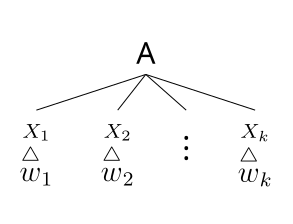
\includegraphics{caso_passo.png}
%			      \psframebox[linestyle=none,framesep=10pt]{%
%				      \pstree{\LFTw{t}{\fontspec{Noto Sans}[Script=Latin]A}}{\pstree{\Tp[edge=none]}{%
%						      \LFTw{t}{\fontspec{Noto Sans}[Script=Latin]$\overset{X_1}{\overset{\triangle}w_1}$}
%						      \LFTw{t}{\fontspec{Noto Sans}[Script=Latin]$\overset{X_2}{\overset{\triangle}w_2}$}
%						      \LFTw{t}{\fontspec{Noto Sans}[Script=Latin]$\vdots$}
%						      \LFTw{t}{\fontspec{Noto Sans}[Script=Latin]$\overset{X_k}{\overset{\triangle}w_k}$}}}}
					\end{center}
					$$A\to_{lm} X_1,X_2,...,X_k$$
					$$x_1\to^*_{lm}w_1 \mbox{ per ipotesi induttiva si ha un albero al più di n livelli}$$
					quindi:
					$$A\to_{lm}X_1,...,X_k\to^*_{lm}w_1,X_2,...,X_k\to^*_{lm}...\to^*_{lm}w_1,...,w_k=w$$
	\end{itemize}
	\begin{example}
		$$E\to I\to Ib\to ab$$
		$$\alpha E\beta\to\alpha I\beta\to \alpha Ib\beta\to \alpha ab\beta,\,\,\,\alpha,\beta\in(V\cup T)^*$$
	\end{example}
\end{proof}
\begin{example}
	Mostro l'esistenza di una derivazione sinistra dell'albero sintattico di $a*(a+b00)$:
	$$E\to^*_{lm}E*E\to^*_{lm}I*E\to^*_{lm}a*E\to^*_{lm}a*(E)\to^*_{lm}a*(E+E)\to^*_{lm}$$
	$$a*(I+E)\to^*_{lm}a*(a+E)\to^*_{lm}a*(a+I)\to^*_{lm}a+(a+I0)\to^*_{lm}a*(a+I00)\to^*_{lm}a*(a+b00)$$
\end{example}
\section{Grammatiche ambigue}
\begin{definition}
	Una grammatica è definita ambigua se esiste una stringa $w$ di terminali che ha più di un albero sintattico
\end{definition}
\begin{example}
	vediamo un esempio:
	\begin{enumerate}
		\item $E\to E+E\to E+E*E$
					ovvero:
					\begin{center}
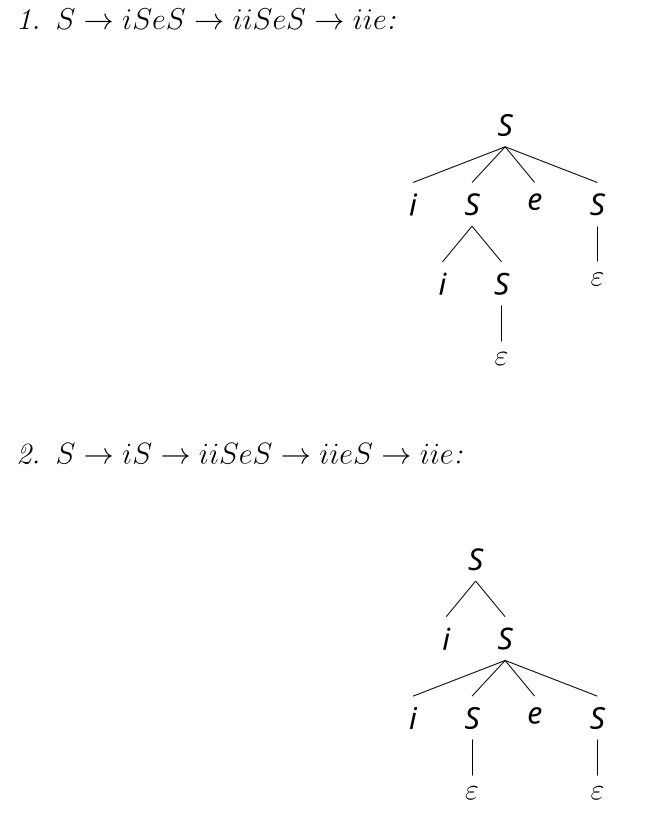
\includegraphics{ambigua1.png}
%			      \psframebox[linestyle=none,framesep=10pt]{%
%				      \pstree{\LFTw{t}{\fontspec{Noto Sans}[Script=Latin]E}}{\pstree{\Tp[edge=none]}{%
%						      \LFTw{t}{\fontspec{Noto Sans}[Script=Latin]E}
%						      \LFTw{t}{\fontspec{Noto Sans}[Script=Latin]+}
%						      \pstree{\LFTw{t}{\fontspec{Noto Sans}[Script=Latin]E}}{\pstree{\Tp[edge=none]}{%
%								      \LFTw{t}{\fontspec{Noto Sans}[Script=Latin]E}
%								      \LFTw{t}{\fontspec{Noto Sans}[Script=Latin]*}
%								      \LFTw{t}{\fontspec{Noto Sans}[Script=Latin]E}}}}}}
					\end{center}
		\item $E\to E*E\to E+E*E$
					ovvero:
					\begin{center}
%			      \psframebox[linestyle=none,framesep=10pt]{%
%				      \pstree{\LFTw{t}{\fontspec{Noto Sans}[Script=Latin]E}}{\pstree{\Tp[edge=none]}{%
%						      \pstree{\LFTw{t}{\fontspec{Noto Sans}[Script=Latin]E}}{\pstree{\Tp[edge=none]}{%
%								      \LFTw{t}{\fontspec{Noto Sans}[Script=Latin]E}
%								      \LFTw{t}{\fontspec{Noto Sans}[Script=Latin]+}
%								      \LFTw{t}{\fontspec{Noto Sans}[Script=Latin]E}}}
%						      \LFTw{t}{\fontspec{Noto Sans}[Script=Latin]*}
%						      \LFTw{t}{\fontspec{Noto Sans}[Script=Latin]E}}}}
					\end{center}
	\end{enumerate}
	si arriva a due stringhe uguali ma con alberi diversi. Introduciamo delle categorie sintatiche, dei vincoli alla produzione delle regole:
	\begin{enumerate}
		\item $E\to T|\, E+T$
		\item $T\to F|\, T+F$
		\item $F\to I|\, (E)$
		\item $I\to a|\,b|\,Ia|,Ib|\,I0|\,I1$
	\end{enumerate}
\end{example}
Possono esserci più derivazioni di una stringa ma l'importante è che non ci siano alberi sintattici diversi. Capire se una CFG è ambigua è un problema indecidibile
\begin{example}
	vediamo un esempio:
	$$S\to \varepsilon|\,SS|\, iS|\, iSeS$$
	con S=statement, i=if e e=else. Considero due derivazioni:
	\begin{enumerate}
		\item $S\to iSeS\to iiSeS\to iie$:
					\begin{center}
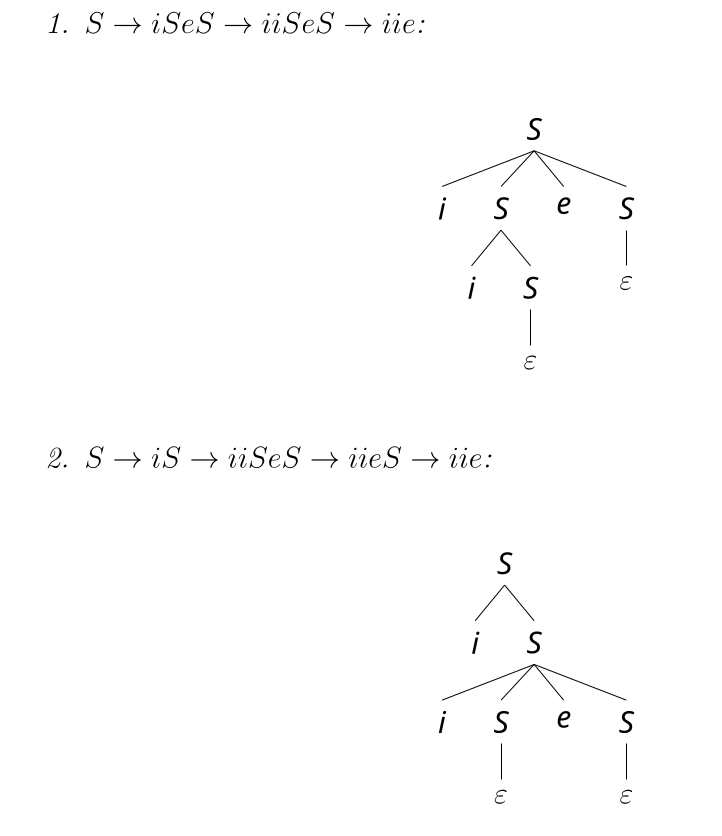
\includegraphics{ambigua2.png}

%			      \psframebox[linestyle=none,framesep=10pt]{%
%				      \pstree{\LFTw{t}{\fontspec{Noto Sans}[Script=Latin]S}}{\pstree{\Tp[edge=none]}{%
%						      \LFTw{t}{\fontspec{Noto Sans}[Script=Latin]i}
%						      \pstree{\LFTw{t}{\fontspec{Noto Sans}[Script=Latin]S}}{\pstree{\Tp[edge=none]}{%
%								      \LFTw{t}{\fontspec{Noto Sans}[Script=Latin]i}
%								      \pstree{\LFTw{t}{\fontspec{Noto Sans}[Script=Latin]S}}{\pstree{\Tp[edge=none]}{%
%										      \LFTw{t}{\fontspec{Noto Sans}[Script=Latin]$\varepsilon$}}}}}
%						      \LFTw{t}{\fontspec{Noto Sans}[Script=Latin]e}
%						      \pstree{\LFTw{t}{\fontspec{Noto Sans}[Script=Latin]S}}{\pstree{\Tp[edge=none]}{%
%								      \LFTw{t}{\fontspec{Noto Sans}[Script=Latin]$\varepsilon$}}}}}}\end{center}
%		\item $S\to iS\to iiSeS\to iieS\to iie$:
%		      \begin{center}
%
%			      \psframebox[linestyle=none,framesep=10pt]{%
%				      \pstree{\LFTw{t}{\fontspec{Noto Sans}[Script=Latin]S}}{\pstree{\Tp[edge=none]}{%
%						      \LFTw{t}{\fontspec{Noto Sans}[Script=Latin]i}
%						      \pstree{\LFTw{t}{\fontspec{Noto Sans}[Script=Latin]S}}{\pstree{\Tp[edge=none]}{%
%								      \LFTw{t}{\fontspec{Noto Sans}[Script=Latin]i}
%								      \pstree{\LFTw{t}{\fontspec{Noto Sans}[Script=Latin]S}}{\pstree{\Tp[edge=none]}{%
%										      \LFTw{t}{\fontspec{Noto Sans}[Script=Latin]$\varepsilon$}}}
%								      \LFTw{t}{\fontspec{Noto Sans}[Script=Latin]e}
%								      \pstree{\LFTw{t}{\fontspec{Noto Sans}[Script=Latin]S}}{\pstree{\Tp[edge=none]}{%
%										      \LFTw{t}{\fontspec{Noto Sans}[Script=Latin]$\varepsilon$}}}}}}}}
					\end{center}
	\end{enumerate}
	Si ha quindi una grammatica ambigua
\end{example}
\begin{theorem}
	Per ogni CFG, con $G=(V, T, P, S)$, per ogni stringa $w$ di terminali si ha che $w$ ha due alberi sintattici distinti sse ha due derivazioni sinistre da S distinte.\\
	Se la grammatica non è ambigua allora esiste un'unica derivazione sinistra da $S$
\end{theorem}
\subsubsection{Linguaggi inerentemente ambigui}
\begin{definition}
	Un linguaggio $L$ è inerentemente ambiguo se tutte le grammatiche CFG per tale linguaggio sono a loro volta ambigue
\end{definition}
\begin{example}
	Sia $L=\{a^nb^nc^md^m|\, n,m\geq 1\}\cup \{a^nbmnc^md^n|\, n,m\geq 1\}$\\
	si ha quindi un CFL formato dall'unione di due CFL. $L$ è inerentemente ambiguo e generato dalla seguente grammatica:
	\begin{itemize}
		\item $S\to AB|\,C$
		\item $A\to aAb|\,ab$
		\item $B\to cBd|\, cd$
		\item $C\to aCd|\, aDd$
		\item $D\to bDc|\, bc$
	\end{itemize}
	si possono avere due derivazioni:
	\begin{enumerate}
		\item $S\to_{lm}AB\to_{lm} aAbB\to_{lm} aabbB\to_{lm}aabbcBd\to_{lm}aabbccdd$
		\item $S\to_{lm} C\to_{lm} aCd\to_{lm}aaBdd\to_{lm}aabBcdd\to_{lm}aabbccdd$
	\end{enumerate}
	a generare problemi sono le stringhe con n=m perché possono essere prodotte in due modi diversi da entrambi i sottolinguaggi. Dato che l'intersezione tra i due sottolinguaggi non è buota si ha che $L$ è ambiguo
\end{example}
\section{Grammatiche Regolari}
Sono le grammatiche che generano i linguaggi regolari (quelli del terzo tipo) che sono casi particolari dei CFL.\\
Si ha la solita grammatica $G = (V, T, P, S)$ con però vincoli su $P$:
\begin{itemize}
	\item $\varepsilon$ si può ottenere solo con $S\to \varepsilon$
	\item le produzioni sono tutte lineari a destra ($A\to aA$ o $A\to a$) o a sinistra ($A\to Ba$ o $A\to a$)
\end{itemize}
\begin{example}
	$I\to a|\,b|\,Ia|\,Ib|\,I0|\,I1$ è una grammatica con le produzioni lineari a sinistra.\\
	Potremmo pensarlo a destra $I\to a|\,b|\,aI|\,bI|\,0I|\,1I$.\\
	Vediamo esempi di produzione con queste grammatiche:
	\begin{itemize}
		\item con $I\to a|\,b|\,Ia|\,Ib|\,I0|\,I1$ possiamo derivare $ab01b0$:
					$$I\to I0\to Ib0\to I1b0\to I01b0\to Ib01b0\to ab01b0$$
		\item con $I\to a|\,b|\,aI|\,bI|\,0I|\,1I$ invece non riusciamo a generare nulla:
					$$I\to 0I\to 0a$$
	\end{itemize}
	definisco quindi un'altra grammatica (con una nuova categoria sintattica):
	$$I\to aJ|\, bJ$$
	$$J\to a|\,b|\,aJ|\,bJ|\,0J|\,1J$$
	che però non mi permette di terminare le stringhe con 0 e 1, la modifico ancora otterdendo:
	$$I\to aJ|\, bJ$$
	$$J\to a|\,b|\,aJ|\,bJ|\,0J|\,1J|\,0|\,1$$
	e questo è il modo corretto per passare da lineare sinistra a lineare destra
\end{example}
\begin{example}
	Sia $G=(\{S\},\{0,1\},P,S)$ con $S\to \varepsilon|\,0|\,1|\,0S|\,1S$. Si ha quindi:
	$$L(G)=\{0,1\}^*$$
	si hanno comunque due proposizioni ridondanti, riducendo trovo:
	$$S\to \varepsilon|\, 0S|\,1S$$
	con solo produzioni lineari a destra. Con produzioni lineari a sinistra ottengo:
	$$S\to \varepsilon|\, S0|\,S1$$
\end{example}
\begin{example}
	Trovo una grammatica lineare destra e una sinistra per $L=\{a^nb^m|\,n,m\geq 0\}$:
	\begin{itemize}
		\item \textbf{lineare a destra:} si ha $G=(\{S,B\},\{a,b\},P,S)$ e quindi:
					$$S\to \varepsilon|\,aS|\,bB$$
					$$B\to bB|\,b$$
					ma non si possono generare stringhe di sole $b$, infatti:
					$$S\to aS\to abB\to abbB\to abbb$$
					ma aggiungere $\varepsilon$ a B \textbf{non è lecito}. posso però produrre la stessa stringa da due derivazioni diverse:
					$$S\to \varepsilon|\,aS|\,bB|\,b$$
					$$B\to bB|\,b$$
					che risulta quindi la nostra lineare a destra
		\item \textbf{lineare a sinistra:} si ha $G=(\{S,A\},\{a,b\},P,S)$ e quindi:
					$$S\to \varepsilon|\,Sb|\,Ab|\,a$$
					$$A\to Aa|\,a$$
	\end{itemize}
\end{example}
\begin{example}
	Trovo una grammatica lineare destra e una sinistra per $L=\{ab^ncd^me|\,n\geq 0\,,m> 0\}$:
	\begin{itemize}
		\item \textbf{lineare a destra:} si ha  si ha $G=(\{S,A,B,E\},\{a,b,c,d,e\},P,S)$ e quindi:
					$$S\to aA$$
					$$A\to bA|\,cB$$
					$$B\to dB|\, dE$$
					$$E\to e$$
		\item \textbf{lineare a sinistra:} si ha  si ha $G=(\{S,X,Y,Z\},\{a,b,c,d,e\},P,S)$ e quindi:
					$$S\to Xe$$
					$$A\to Xd|\,Yd$$
					$$B\to Zc$$
					$$E\to a|\,Zb$$
	\end{itemize}
	quindi se per esempio ho la stringa "ciao" si ha:
	\begin{itemize}
		\item \textbf{lineare a destra:}
					$$S\to Ao$$
					$$A\to Ba$$
					$$B\to Ei$$
					$$E\to c$$
		\item \textbf{lineare a sinistra:}
					$$S\to cA$$
					$$A\to iB$$
					$$B\to aE$$
					$$E\to o$$
	\end{itemize}
\end{example}
\begin{example}
	A partire da $G=(\{S,T\},\{0,1\},P,S)$ con:
	$$S\to\varepsilon|\,0S|\,1T$$
	$$T\to 0T|\,1S$$

	trovo come è fatto $L(G)$:
	$$L(G)=\{w\in\{0,1\}^*|\, w \mbox{ ha un numero di 1 pari}\}$$
\end{example}
\begin{example}
	fornire una grammatica regolare a destra e sinistra per:
	$$L=\{w\in\{0,1\}^*|\, w \mbox{ ha almeno uno 0 o almeno un 1}\}$$
	Si ah che tutte le stringhe tranne quella vuota ciontengono uno 0 o un 1
	quindi  $G=(\{S\},\{0,1\},P,S)$:
	\begin{itemize}
		\item \textbf{lineare a destra:}
					$$S\to 0|\,1|\,0S|\,1S$$
		\item \textbf{lineare a sinistra:}
					$$S\to 0|\,1|\,S0|\,S1$$
	\end{itemize}
\end{example}



Vediamo ora un esempio di \textit{Context Free Language (CFL)}, costruito a partire da una \textit{Context Free Grammar (CFG)}:
\begin{example}
	Sia $\Sigma=\{0, 1\}$ e $L_{pal}="stringhe\,\, palindrome\,\, binarie"$.
	Quindi, per esempio, $0110\in L,\,\, 11011\in L$ ma $10010\not\in L$. Si ha che $\varepsilon$, la stringa vuota, appartiene a $L$. Diamo una definizione ricorsiva:
	\begin{itemize}
		\item \textbf{base:} $\varepsilon,\, 0\,\ 1\in L_{pal}$
		\item \textbf{passo:} se $w$ è palindroma allora $0w0$ è palindromo e $1w1$ è palindromo
	\end{itemize}
	una variabile generica $S$ può sottostare alle \textit{regole di produzione} di una certa grammatica. In questo caso si ha uno dei seguenti:
	$$S\to\varepsilon,\, S\to 0,\, S\to 1,\, S\to 0S0,\, S\to 1S1$$
\end{example}


riprendiamo l'esempio sopra:
\begin{example}
	$$G_{pal}=(V=\{S\},\, T=\{0, 1\},\, P,\, S)$$
	con:
	$$P=\{S\to\varepsilon,\, S\to 0,\, S\to 1,\, S\to 0S0,\, S\to 1S1\}$$
	Si può ora costruire un algoritmo per creare una stringa palindroma a partire dalla grammatica $G$:
	$$\underbrace{S}_{\mbox{start}}\underbrace{\to}_{\mbox{applico una regola}} 1S1 \to 01S10\to \underbrace{01010}_{\mbox{sostituisco variabile}}$$

	con $S,\, 1S1\,\, e\,\, 01S10$ che sono \textit{forme sentenziali}. Posso così ottenere tutte le possibili stringhe. Esiste anche una forma abbreviata:
	$$S\to \varepsilon|o|1|0S0|1S1$$
	Non si fanno sostituzioni in parallelo, prima una $S$ e poi un'altra
\end{example}


\section{Automi a Pila}\label{sec:automi-pila}

	Si introduce un nuovo tipo di automa, il PDA (push down automata) che può essere pensato come un $\varepsilon-NFA$ col supporto di una pila (stack):
	\begin{center}
	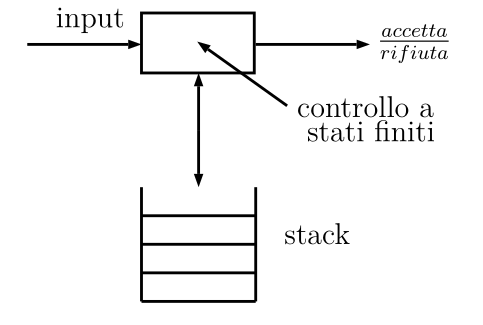
\includegraphics{2025-01-16_14-59.png}
		% \psscalebox{1.0 1.0} % Change this value to rescale the drawing.
		% {
		% 	\begin{pspicture}(0,-2.04)(5.83,2.04)
		% 		\psframe[linecolor=black, linewidth=0.04, dimen=outer](3.2,2.04)(1.58,1.16)
		% 		\psline[linecolor=black, linewidth=0.04, arrowsize=0.05291667cm 2.0,arrowlength=1.4,arrowinset=0.0]{->}(0.0,1.58)(1.6,1.58)
		% 		\psline[linecolor=black, linewidth=0.04, arrowsize=0.05291667cm 2.0,arrowlength=1.4,arrowinset=0.0]{->}(3.2,1.58)(4.8,1.58)
		% 		\psline[linecolor=black, linewidth=0.04, arrowsize=0.05291667cm 2.0,arrowlength=1.4,arrowinset=0.0]{->}(2.4,0.38)(2.4,-0.42)
		% 		\psline[linecolor=black, linewidth=0.04, arrowsize=0.05291667cm 2.0,arrowlength=1.4,arrowinset=0.0]{->}(2.4,0.38)(2.4,1.18)
		% 		\psline[linecolor=black, linewidth=0.04](1.6,-0.42)(1.6,-2.02)
		% 		\psline[linecolor=black, linewidth=0.04](3.2,-2.02)(1.6,-2.02)
		% 		\psline[linecolor=black, linewidth=0.04](3.2,-2.02)(3.2,-0.42)
		% 		\psline[linecolor=black, linewidth=0.04](1.6,-0.82)(3.2,-0.82)
		% 		\psline[linecolor=black, linewidth=0.04](1.6,-1.22)(3.2,-1.22)
		% 		\psline[linecolor=black, linewidth=0.04](1.6,-1.62)(3.2,-1.62)
		% 		\rput[bl](4.9,1.32){$\frac{accetta}{rifiuta}$}
		% 		\rput[bl](0.4,1.74){input}
		% 		\rput[bl](3.78,0.22){ stati finiti}
		% 		\rput[bl](3.6,-1.22){stack}
		% 		\psline[linecolor=black, linewidth=0.04, arrowsize=0.05291667cm 2.0,arrowlength=1.4,arrowinset=0.0]{->}(3.64,0.72)(2.38,1.62)
		% 		\rput[bl](3.78,0.56){controllo a}
		% 	\end{pspicture}
		% }
	Tikz
	\end{center}
	e viene definito un PDA $P$ come:
	$$P=(Q,\Sigma,\Gamma,\delta,q_0,z_0,F)$$
	con;
	\begin{itemize}
		\item $Q$: insieme finito e non vuoto di stati
		\item $\Sigma$: alfabeto di simboli di input
		\item $\Gamma$: alfabeto di simboli di stack
		\item $q_0\in Q$: stato iniziale
		\item $z_0\in \Gamma\backslash \Sigma$: simbolo iniziale dello stack
		\item $F\in Q$: insieme degli stati accettanti o finali
	\end{itemize}
	si ha che:
	$$\delta:Q\times(\Sigma\cup\{\varepsilon\}\times \Gamma\to 2^{Q\times \Gamma^*}$$
	quindi:
	$$\delta(q_0,a,X)=\{(p_1,X_1),(p_2,X_2),...\}\,insieme\,\,\,finito\,\,p_i\in Q\,\,X_i\in \Gamma^*$$
	si hanno dei casi particolari:
	\begin{itemize}
		\item lo stato $p$ potrebbe coincidere con $Q$ e si avrebbe un cappio
		\item se $\Gamma=\varepsilon$ si ha il pop di $X$ dallo stack
		\item se $\Gamma=X$ si lascia lo stack invariato
		\item se $\Gamma=Y\neq X$ si ha la sostituzione di $X$ con $Y$ in cima allo stack
		\item se $\Gamma$ è una stringa di simboli si ha il la rimozione di $X$ dallo stack e l'aggiunta a uno a uno dei simboli nello stack
	\end{itemize}
	\newpage
	\begin{example}
		Trovo PDA per il linguaggio delle stringhe binarie  palindrome di lunghezza pari: $L=\{ww^R|w\in\{0,1\}^*\}$. Con $R$ che indica rovesciato\\
		Si ha la CFG $G=(\{P\},\{0,1\},Prod,P)$ tale che:
		$$P\to 0P0|1P1|\varepsilon$$
		si hanno quindi tre stati:
		\begin{itemize}
			\item $q_0$ che è quello iniziale che legge $w$ e spinge i dati sullo stack
			\item $q_1$ che letta $w$ legge i simboli di $wR$ e li confronta con quelli dello stack
			\item $q_2$ sarà la stringa accettata
		\end{itemize}
		descriviamo formalmente l'automa con la funzione di transizione $\delta$.
		PDA $P=(\{q_0,q_1,q_2\},\{0,1\}, \{o,1,z_0\},\delta,q_0,z_0,\{q_2\})$
		ovvero:
		$$\delta(q_0,0,z_0)=\{(q_0,1z_0)\}$$
		$$\delta(q_0,1,z_0)=\{(q_0,0z_0)\}$$
		$$\delta(q_0,0,0)=\{(q_0,00)\}$$
		$$\delta(q_0,0,1)=\{(q_0,01)\}$$
		$$\delta(q_0,1,0)=\{(q_0,10)\}$$
		$$\delta(q_0,1,1)=\{(q_0,11)\}$$
		$$\delta(q_0,\varepsilon,z_0)=\{(q_0,z_0)\}$$
		$$\delta(q_0,\varepsilon,0)=\{(q_0,0)\}$$
		$$\delta(q_0,\varepsilon,1)=\{(q_0,1)\}$$
		$$\delta(q_1,0,0)=\{(q_1,\varepsilon)\}$$
		$$\delta(q_2,1,1)=\{(q_1,\varepsilon)\}$$
		$$\delta(q_2,\varepsilon,z_0)=\{(q_2,0z_0)\}$$
		\newpage
		otteniamo il seguente PDA:
		\begin{center}
			\begin{tikzpicture}[shorten >=1pt,node distance=3cm,on grid,auto]
				\node[state, initial] (q_0) {$q_0$};
				\node[state] (q_1) [right=of q_0] {$q_1$};
				\node[state, accepting] (q_2) [right =of q_1] {$q_2$};
				\path[->]
				(q_0) edge node [align=center] {$\varepsilon,0/0$\\$\varepsilon,1/1$\\$\varepsilon,z_0/z_0$} (q_1)
				edge [loop below] node [align=center] {$0,z_0/0z_0$\\$1,z_0/1z_0$\\$0,0/00$\\$0,1/01$\\$1,0/10$\\$1,1/11$} ()
				(q_1) edge [loop below] node [align=center] {$0,0/\varepsilon$\\$1,1/\varepsilon$} ()
				edge  node [align=center] {$\varepsilon,z_0/z_0$} (q_2);
			\end{tikzpicture}
		\end{center}
		e si definisce questa notazione per gli archi:
		$$(p,\alpha)\in\delta(q,a,X)$$
		\begin{center}
			\begin{tikzpicture}[shorten >=1pt,node distance=3cm,on grid,auto]
				\node[state, initial] (q_0) {$q_0$};
				\node[state] (q_1) [right=of q_0] {$q_1$};
				\path[->]
				(q_0) edge node [align=center] {$a,X/\alpha$} (q_1);
			\end{tikzpicture}
		\end{center}
	\end{example}
	analizziamo meglio i PDA. Si ha che la \textbf{descrizione istantanea (ID)} di un PDA è una tripla:
	$$ID:(q,w,\gamma)$$
	con $q\in Q$ stato attuale $w\in\Sigma^*$ input rimanente e $\gamma\in\Gamma^*$ contenuto attuale dello stack.\\
	Definiamo ora il concetto di \textbf{mossa in un passo}
	dato $P=(Q,\Sigma,\Gamma,\delta,q_0,z_0,F)$ la mossa è una relazione $\vdash_p$:
	$$(p,\alpha)\in\delta(q,a,X)\,\,allora\,\,\forall w\in\Sigma^*\,\,e\,\, \forall\beta\in\Gamma^*\to (q,aw,X\beta)\vdash(p,w,\alpha\beta$$
	e
	$$(p,\alpha)\in\delta(q,\varepsilon,X)\,\,allora\,\,\forall w\in\Sigma^*\,\,e\,\, \forall\beta\in\Gamma^*\to (q,w,X\beta)\vdash(p,w,\alpha\beta)$$
	\newpage
	ora possiamo anche definire la relazione con 0 o più mosse
	in forma induttiva $\stackrel{*}{\vdash_p}$:
	\begin{itemize}
		\item \textbf{caso base:} $\forall ID\,\,I, I \stackrel{*}{\vdash} I$
		\item \textbf{caso passo:} $I \stackrel{*}{\vdash} J$ se $\exists ID\,\,K$ tale che $ I\vdash K \,\,e\,\, K \stackrel{*}{\vdash} J$
	\end{itemize}
	vediamo un esempio con un PDA che accetta $ww^R|\,w\in\{0,1\}^*$:
	\begin{center}
		\begin{tikzpicture}[shorten >=1pt,node distance=3cm,on grid,auto]
			\node[state, initial] (q_0) {$q_0$};
			\node[state] (q_1) [right=of q_0] {$q_1$};
			\node[state, accepting] (q_2) [right =of q_1] {$q_2$};
			\path[->]
			(q_0) edge node [align=center] {$\varepsilon,0/0$\\$\varepsilon,1/1$\\$\varepsilon,z_0/z_0$} (q_1)
			edge [loop below] node [align=center] {$0,z_0/0z_0$\\$1,z_0/1z_0$\\$0,0/00$\\$0,1/01$\\$1,0/10$\\$1,1/11$} ()
			(q_1) edge [loop below] node [align=center] {$0,0/\varepsilon$\\$1,1/\varepsilon$} ()
			edge  node [align=center] {$\varepsilon,z_0/z_0$} (q_2);
		\end{tikzpicture}
	\end{center}
	e prendiamo la stringa $1111$:\\
	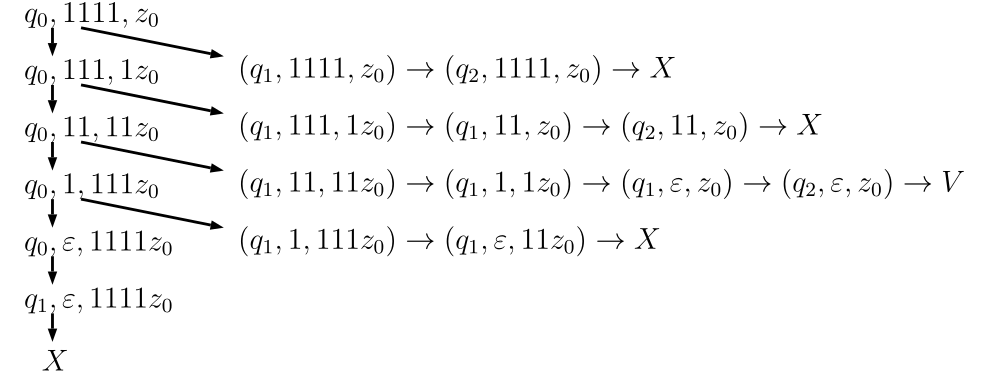
\includegraphics{2025-01-16_15-01.png}
	% \\
	% \psscalebox{1.0 1.0} % Change this value to rescale the drawing.
	% {
	% 	\begin{pspicture}(0,-2.51)(3.08,2.51)
	% 		\rput[bl](0.0,2.29){$q_0,1111,z_0$}
	% 		\rput[bl](0.0,1.49){$q_0,111,1z_0$}
	% 		\rput[bl](0.0,0.69){$q_0,11,11z_0$}
	% 		\rput[bl](0.0,-0.11){$q_0,1,111z_0$}
	% 		\rput[bl](0.0,-0.91){$q_0,\varepsilon,1111z_0$}
	% 		\rput[bl](0.0,-1.71){$q_1,\varepsilon,1111z_0$}
	% 		\rput[bl](0.25,-2.51){$X$}
	% 		\rput[bl](3.0,1.49){$(q_1,1111,z_0)\to(q_2,1111,z_0)\to X$}
	% 		\rput[bl](3.0,0.69){$(q_1,111,1z_0)\to (q_1,11,z_0)\to(q_2,11,z_0)\to X$}
	% 		\rput[bl](3.0,-0.11){$(q_1,11,11z_0)\to(q_1,1,1z_0)\to(q_1,\varepsilon,z_0)\to(q_2,\varepsilon,z_0)\to V$}
	% 		\rput[bl](3.0,-0.91){$(q_1,1,111z_0)\to(q_1,\varepsilon,11z_0)\to X$}
	% 		\psline[linecolor=black, linewidth=0.04, arrowsize=0.05291667cm 2.0,arrowlength=1.4,arrowinset=0.0]{->}(0.4,2.29)(0.4,1.89)
	% 		\psline[linecolor=black, linewidth=0.04, arrowsize=0.05291667cm 2.0,arrowlength=1.4,arrowinset=0.0]{->}(0.4,1.49)(0.4,1.09)
	% 		\psline[linecolor=black, linewidth=0.04, arrowsize=0.05291667cm 2.0,arrowlength=1.4,arrowinset=0.0]{->}(0.4,0.69)(0.4,0.29)
	% 		\psline[linecolor=black, linewidth=0.04, arrowsize=0.05291667cm 2.0,arrowlength=1.4,arrowinset=0.0]{->}(0.4,-0.11)(0.4,-0.51)
	% 		\psline[linecolor=black, linewidth=0.04, arrowsize=0.05291667cm 2.0,arrowlength=1.4,arrowinset=0.0]{->}(0.4,-0.91)(0.4,-1.31)
	% 		\psline[linecolor=black, linewidth=0.04, arrowsize=0.05291667cm 2.0,arrowlength=1.4,arrowinset=0.0]{->}(0.4,-1.71)(0.4,-2.11)
	% 		\psline[linecolor=black, linewidth=0.04, arrowsize=0.05291667cm 2.0,arrowlength=1.4,arrowinset=0.0]{->}(0.8,1.49)(2.8,1.09)
	% 		\psline[linecolor=black, linewidth=0.04, arrowsize=0.05291667cm 2.0,arrowlength=1.4,arrowinset=0.0]{->}(0.8,2.29)(2.8,1.89)
	% 		\psline[linecolor=black, linewidth=0.04, arrowsize=0.05291667cm 2.0,arrowlength=1.4,arrowinset=0.0]{->}(0.8,0.69)(2.8,0.29)
	% 		\psline[linecolor=black, linewidth=0.04, arrowsize=0.05291667cm 2.0,arrowlength=1.4,arrowinset=0.0]{->}(0.8,-0.11)(2.8,-0.51)
	% 	\end{pspicture}
	% }
	\\
	chiamiamo \textbf{computazione }una sequenza di mosse, non necessariamente di successo. Si hanno alcune proprietà:
	\begin{itemize}
		\item se una se una sequenza di ID è lecita per un PDA P allora è lecita anche la sequenza di Id ottenuta concatenando $w\in\Sigma^*$ in ogni ID
		\item se una se una sequenza di ID è lecita per un PDA P e resta una coda di input non consumata allora posso rimuovere tale coda in ogni ID e ottenere un'altra sequenza lecita
		\item se una se una sequenza di ID è lecita per un PDA P allora  è lecita la sequenza ottenuta aggiungendo $\gamma\in\Gamma^*$ in coda alla terza sequenza di ogni ID
	\end{itemize}
	del resto però:
	$$(q,Xw,\alpha\gamma) \stackrel{*}{\vdash_p} (p,Yw,\beta\gamma)\not\to (q,X,\alpha) \stackrel{*}{\vdash}(p,y,\beta),\,\,x,w,y\in\Sigma^*\,\,\alpha,\beta,\gamma\in\Gamma^*$$
	per queste proprietà valgono i seguenti teoremi:
	\begin{theorem}
		per la seconda:
		Se $P=(Q,\Sigma,\Gamma,\delta,q_0,z_0,F)$ è un PDA e $(q,Xw,\alpha) \stackrel{*}{\vdash_p} (p,Yw,\beta)$ allora vale anche:
		$$(q,X,\alpha) \stackrel{*}{\vdash_p} (p,Y,\beta)$$
	\end{theorem}
	\begin{theorem}
		per la prima e la terza:
		Se $P=(Q,\Sigma,\Gamma,\delta,q_0,z_0,F)$ è un PDA e $(q,X,\alpha) \vdash_p^* (p,Y,\beta)$ allora:
		$$\forall\gamma\in\Gamma^*\,\,\,vale\,\,\,anche\,\,\,(q,Xw,\alpha\gamma) \vdash_p^* (p,Yw,\beta\gamma)$$
	\end{theorem}
	Si definiscono due modalità di accettazione per i PDA:
	\begin{enumerate}
		\item \textbf{per stato finale:} sia $P=(Q,\Sigma,\Gamma,\delta,q_0,z_0,F)$ si ha che:
		      $$L(P)=\{w\in\Sigma^*|\,(q_0,w,z_0) \vdash_p^* (q,\varepsilon,\alpha)\}$$
		      con $q\in F$ e $\forall \alpha\in \Gamma^*$
		\item \textbf{per stack vuoto:} sia $P=(Q,\Sigma,\Gamma,\delta,q_0,z_0,F)$ si ha che:
		      $$N(P)=\{w\in\Sigma^*|\,(q_0,w,z_0) \vdash_p^* (q,\varepsilon,\varepsilon)\}$$
		      con $q\in Q$ e in questo caso l'insieme degli stati finali $F$ non ha alcuna influenza
	\end{enumerate}
	In realtà si ha che la classe di linguaggi accettati dai PDA per stato finale è uguale a quella per stack vuoto, anche se passare da un tipo all'altro di PDA è complesso. SI ha il seguente teorema per la trasformazione:
	\begin{theorem}
		se $L=N(P_N)$ per un PDA  $P_N=(Q,\Sigma,\Gamma,\delta,q_0,z_0,F)$ allora $\exists \,\,PDA\,\,P_F\,\,\,tale\,\,\,che\,\,\,L=L(P_F)$
	\end{theorem}
	\begin{proof}
		Sia $x_0\in\Gamma$, che indica la fine dello stack di $P_F$. Si ha:
		$$\delta(p_0,\varepsilon,x_0)=\{(q_0,z_0x_0\}$$
		e:
		$$\forall q\in Q,\,\forall a\in\Sigma\cup\{\varepsilon\},,\forall y\in\Sigma:\,\,\delta_F(q,a,y)\mbox{ contiene tutte le coppie di }\delta_N(q,a,y)$$
		$$\forall q\in Q,\delta_F(q,\varepsilon,x_0)=\{(P_F,\varepsilon)\}$$
		quindi graficamente:

		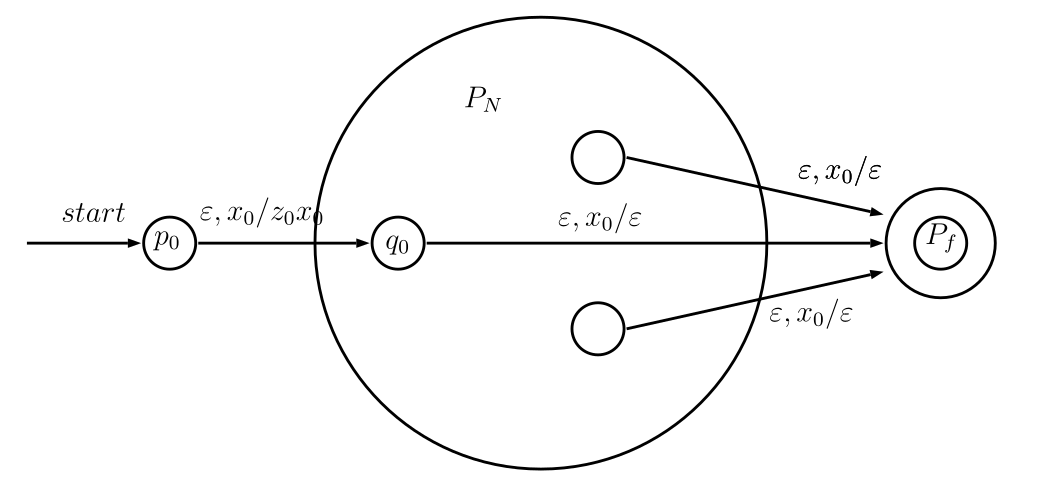
\includegraphics{2025-01-16_15-03.png}
		Bisogna dimostrare che effettivamente $w\in L(P_F)\longleftrightarrow\in N(P_N)$.\\
		se $w\in N(P_N)$ $\exists$ una sequenza di $ID\,\,\,(q_0,w,z_0)\vdash_{P_N}^*(q,\varepsilon,\varepsilon)$ per un qualche $q\in Q$:
		$$(q_0,w,z_0x_0)\vdash_{P_N}^*(q,\varepsilon,x_0)$$
		inoltre:
		$$(q_0,w,z_0x_0)\vdash_{P_F}^*(q,\varepsilon,x_0)$$
		e quindi:
		$$(p_0,w,x_0)\vdash_{P_F}(q_0,w,z_0x_0)\vdash_{P_F}^*(q,\varepsilon,x_0)\vdash_{P_F}(P_F,\varepsilon,\varepsilon)$$
		solo se togliendo il primo e l'ultimo passo di $P_F$ ripercorro all'indietro quanto scritto sopra.
	\end{proof}
	\begin{example}
		trasformazione da accettante per stack vuoto a accettante per stato finale. Siano:
		$$\Sigma=\{i,e\}$$
		$$P_n=(\{q\}, \{i,e\},\{Z\},\delta_M,q,Z)$$
		$$\delta_N(q,i,Z)=\{(q,ZZ)\}$$
		$$\delta_N(q,e,Z)=\{(q,\varepsilon)\}$$
		quindi:
		\begin{center}
			\begin{tikzpicture}[shorten >=1pt,node distance=3cm,on grid,auto]
				\node[state, initial] (q_0) {$q$};
				\path[->]
				(q_0) edge [loop above] node [align=center] {$i,Z/ZZ$\\$e,Z/\varepsilon$} ();
			\end{tikzpicture}
		\end{center}
		quindi inseriamo una $Z$ quando leggiamo $i$ e ne rimuoviamo una se leggiamo $e$ e si parte con una $Z$ nello stack.\\
		Costruisco ora il PDA $P_F$ che accetta lo stesso linguaggio ma per stato finale, introduco lo stato iniziale $p$ e quello  accettante $r$, uso $x_0$ come segnale della fine dello stack:
		\begin{center}
			\begin{tikzpicture}[shorten >=1pt,node distance=3cm,on grid,auto]
				\node[state, initial] (q_0) {$p$};
				\node[state] (q_1) [right=of q_0] {$q$};
				\node[state, accepting] (q_2) [right =of q_1] {$r$} ;
				\path[->]
				(q_0) edge  node [align=center] {$\varepsilon x_0/zx_0$} (q_1)
				(q_1) edge node {$\varepsilon,x_0/\varepsilon$} (q_2)
				edge [loop above] node [align=center] {$i,Z/ZZ$\\$e,Z/\varepsilon$} ();
			\end{tikzpicture}
		\end{center}
		e si ha formalmente:
		$$P_F=(\{p,q,r\}, \{i,e\},\{Z,x_0\},\delta_F,p,x_0,\{r\})$$
		con $\delta_F$ che rappresenta le seguenti quattro regole:
		\begin{enumerate}
			\item $\delta_F(p,\varepsilon,x_0)=\{(q,Zx_0)\}$ regola che fa partire $P_F$ con $x_o$ come segnalatore dello stack
			\item $\delta_F(p,i,Z)=\{(q,ZZ)\}$ regola che inserisce $Z$ quando si ha $i$ simulando $P_N$
			\item $\delta_F(p,e,Z)=\{(q,Z\varepsilon)\}$ regola che rimuove $Z$ quando si ha $e$ simulando $P_N$
			\item $\delta_F(p,e,x_0)=\{(r,\varepsilon)\}$ regola che permette a $P_F$ di accettare quando $P_N$ esaurisce lo stack
		\end{enumerate}
	\end{example}
	Si può anche effettuare la trasformazione inversa:
	\begin{theorem}
		Sia $P_F=(Q,\Sigma,\Gamma,\delta_f,q_0,Z_0,F)$.\\
		Si aggiunge una transizione $\varepsilon$  a un nuovo stato $p$ da ogni accettante di $P_F$. quando si ha $p$ $P_N$ svuota lo stack senza consumare input. Quindi se $P:F$ entra in uno stato accettante dopo aver consumato l'input $w$, $P_N$ svuota lo stack dopo aver consumato $w$. Per evitare che si svuoti lo stack per una stringa non accettata uso $x_0$ per indicare il fondo dello stack. Il nuovo $P_N$ parte da $p_0$ che ha il solo scopo di inserire il simbolo iniziale di $P_F$ e passare al suo stato iniziale. Si ottiene quindi:
		\begin{center}
		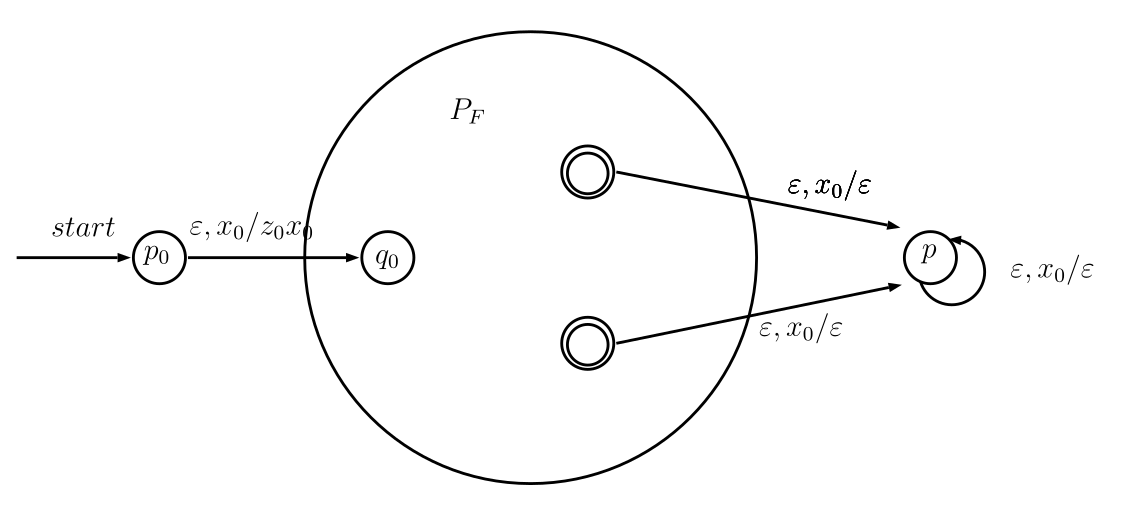
\includegraphics{2025-01-16_15-04.png}
		\end{center}
		e si ha formalmente:
		$$P_F=(Q\cup\{p_0,p\}, \Sigma,\Gamma\cup\{x_0\},\delta_N,p_0,x_0)$$
		dove $\delta_N$ è così definita:
		\begin{enumerate}
			\item $\delta_N(p_0,\varepsilon,x_0)=\{(q_0,Z_0x_0)\}$ inserisce il simbolo iniziale di $P_F$ nello stack e va allo stato iniziale di $P_F$
			\item $\forall q\in Q$ ogni simbolo di input $a\in\Sigma$, compreso l'input vuoto, e $\forall y\in \Gamma$, $\delta_N(q,a,y)$  contiene tutte le coppie di $\delta_F(q,a,y)$. Quindi $P_N$ simula $P_F$
			\item per tutti gli stati accettanti $q\in F$ e i simboli di stack $y\in\Gamma$, compreso $x_0$, si ha che $\delta_N(q,\varepsilon,y)$ contiene $(p,\varepsilon)$, quindi ogni volta che $P_F$ accetta $P_N$ inizia scaricare lo stack senza consumare ulteriori input
			\item per tutti  i simboli di stack $y\in\Gamma$, compreso $x_0$, si ha che $\delta_N(q,\varepsilon,y)=\{(p,\varepsilon)\}$, quindi giunti allo stato $p$, ovvero quando $P_F$ ha accettato, $P_N$ elimina ogni simbolo nel suo stack fino a svuotarlo
		\end{enumerate}
		inoltre formalmente voglio dimostrare che:
		$$w\in L(P_F)\to w\in N(P_N)$$
		e quindi ho le seguenti mosse:
		$$(q_0,w,z_0)\vdash_{P_F}^*(q,\varepsilon,\alpha)\,\,q\in F,\,\,\alpha\in\Gamma^*$$
		$$(p_o,w,x_0)\vdash(q_0,w,z_0x_0)\vdash_{P_N}^*(q,\varepsilon,\alpha,x_0)\vdash_{P_N}^*(p,\varepsilon,\varepsilon)$$
	\end{theorem}
	\begin{example}
		si ha una CFG $G=(\{i,e\},\{a,b,0,1,*,+,(,)\},P,E)$
		con:
		$$P:I\to a|b|Ia|Ib|I0|I1$$
		$$\,\,E\to E+E|E*E|(E)$$
		si ha il PDA $P_G=(\{q\},\Sigma,\Sigma\cup\{i,e\},\delta,q,E)$:
		\begin{center}
			\begin{tikzpicture}[shorten >=1pt,node distance=3cm,on grid,auto]
				\node[state, initial] (q_0) {$q$};
				\path[->]
				(q_0) edge [loop above] node [align=center] {$\mbox{ }$} ();
			\end{tikzpicture}
		\end{center}
		si ha quindi:
		$$\delta(q,\varepsilon, i)=\{(q,a),(q,b),(q,Ia),(q,Ib),(q,I0),(q,I1)\}$$
		$$\delta(q,\varepsilon, E)=\{(q,I),(q,E+E),(q,E*E),(q,I(E))\}$$
		$$\delta(q,a,a)=\{(q,\varepsilon)\}$$
		$$\delta(q,b,b)=\{(q,\varepsilon)\}$$
		$$\cdots=\{(q,\varepsilon)\}$$
		quindi si ha:
		$$E\to E+E\to i+E\to a+(E)\to a+(i)\to a+(i0)\to a+(b0)$$
		$$(q, a+(b0),E)\vdash (q, a+(b0),E+E)\vdash (q, a+(b0),i+E)\vdash (q, a+(b0),a+E)$$
		$$\vdash (q, +(b0),+E)\vdash (q, (b0),E)\vdash (q, (b0),(E))\vdash (q, b0),E))$$
		$$\vdash (q, b0),i))\vdash (q, b0),i0))\vdash (q, b0),b0)\vdash (q, 0),0))$$
		$$\vdash (q, ),))\vdash (q, \varepsilon,\varepsilon)$$
	\end{example}
	questo esempio è generalizzabile ad ogni CFG


	\begin{theorem}
		sia $G=(V,T,P,S)$ una CFG:
		$$\exists\,\, PDA\,\,Q=(\{q\},T,V\cup T,\delta,q,S)\mbox{ tale che }N(Q)=L(G)$$
		$$\forall A\in V\,\,\delta(q,\varepsilon,A)=\{(q,\beta)|\,A\to B\mbox{ e' una produzione di G}\}$$
		$$\forall a\in T\,\,\delta(q,a,a)=\{(a,\varepsilon)\}$$
	\end{theorem}
	Questo dimostra che ogni CFL può essere accettato da un PDA accettante per stack vuoto. Per il teorema visto in precedenza, posso sempre costruire un altro PDA accettante per stati finale. I PDA accettano tutti e soli i linguaggi CF. Mostrare che accettano solo linguaggi di tipo 2 è complicato.\\
	Un tipo di PDA interessante, soprattutto per i parse, è il PDA deterministico, il \textbf{DPDA}.\\
	Un PDA $P=(Q,\Sigma,\Gamma,\delta,q_0,z_0,F)$ è deterministico se:
	\begin{enumerate}
		\item $|\delta(q,a,x)|\leq 1$ $\forall q\in Q,\forall a\in\Sigma\cup\{\varepsilon\},\forall x\in \Gamma$
		\item se $|\delta(q,a,x)|\neq 0$ per qualche $a\in \Sigma$ allora $|\delta(q,\varepsilon,x)|=0$
	\end{enumerate}
	\begin{example}
		abbiamo il linguaggio $L_{wcw^R}=\{wcw^R|\,w\in\{0,1\}^*\}$\\
		Gli automi a pila deterministici non riconosco tutti i CFL, ma solo una classe strettamente più piccola. Ad esempio non potrebbero riconoscere il linguaggio delle palindrome senza "il segnalibro" c. SI ha quindi:
		\begin{center}
			\begin{tikzpicture}[shorten >=1pt,node distance=3cm,on grid,auto]
				\node[state, initial] (q_0) {$q_0$};
				\node[state] (q_1) [right=of q_0] {$q_1$};
				\node[state, accepting] (q_2) [right =of q_1] {$q_2$} ;
				\path[->]
				(q_0) edge [loop above] node [align=center] {$0,z_0/0z_0$\\$1,z_0/1z_0$\\$0,0/00$\\$0,1/01$\\$1,0/10$\\$1,1/11$} ()
				edge node [align=center] {$c,z_0/0z_0$\\$c,0/0$\\$c,1/1$} (q_1)
				(q_1) edge node {$\varepsilon,z_0/z_0$} (q_2)
				edge [loop above] node [align=center] {$0,0/\varepsilon$\\$1,1/\varepsilon$} ();
			\end{tikzpicture}
		\end{center}
		quindi:
		\begin{center}
		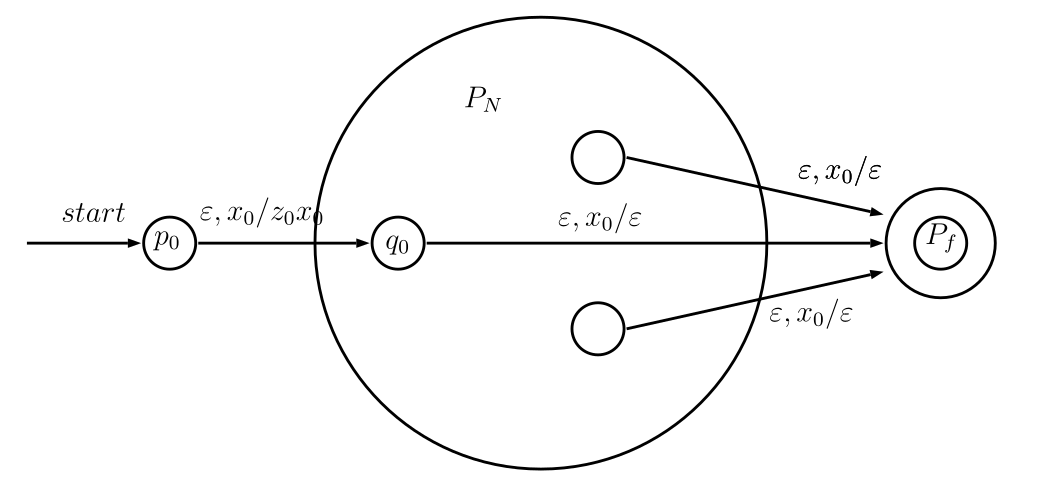
\includegraphics{2025-01-16_15-03.png}
			% \psscalebox{1.0 1.0} % Change this value to rescale the drawing.
			% {
			% 	\begin{pspicture}(0,-2.0)(7.6,2.0)
			% 		\psframe[linecolor=black, linewidth=0.04, dimen=outer](7.6,2.0)(0.0,-2.0)
			% 		\psframe[linecolor=black, linewidth=0.04, dimen=outer](4.8,0.8)(0.8,-1.2)
			% 		\psframe[linecolor=black, linewidth=0.04, dimen=outer](2.4,0.0)(1.2,-0.8)
			% 		\rput[bl](0.4,1.6){CFL}
			% 		\rput[bl](1.46,-0.52){REG}
			% 		\rput[bl](3.68,0.28){DPDA}
			% 		\rput[bl](3.18,1.18){PDA per stato finale}
			% 		\rput[bl](3.2,1.6){PDA per stack vuoto}
			% 		\rput[bl](3.42,-0.86){$Lwcw^R$}
			% 		\rput[bl](5.96,-1.5){$Lww^R$}
			% 	\end{pspicture}
			% }
		\end{center}
	\end{example}
	si ha infatti il seguente teorema:
	\begin{theorem}
		$L\in REG\to\exists PDA\,\,P\,\,tale\,\,che\,\,L=L(P)$
	\end{theorem}
	\begin{proof}
		$$L\in REG\to\exists DFA\,\,A=(Q,\Sigma,\delta_A,q_0,F)\,\,tale\,\,che\,\, L=L(A)$$
		costruisco il DPDA $P=(Q,\Sigma,\{z_0\},\delta_p,q_0,z_0,F)$ con:
		$$\delta_p(q,a,z_0)=\{p,z_0\}\,\,\forall p,q\in Q\,\,tali\,\,che\,\,\delta_A(q,a)=0$$
		vale:
		$$(q_0,w,z_0)\stackrel{A}{\vdash_p}(p,\varepsilon,z_0)\longleftrightarrow \stackrel{\wedge}{\delta_A}(q_0,w)=p$$
	\end{proof}
	si ha inoltre il seguente teorema:
	\begin{theorem}
		$L$ è $N(P)$ per un DPDA $P$ sse $L$ è $L(P^{'})$ per un DPDA $P^{'}$ e $L$ ha le proprietà di prefisso \textbf{prefix-free}
	\end{theorem}
	definiamo così la proprietà di prefisso:
	$$\not\exists x,y\in L\,\,tali\,\,che\,\,x\neq y\,\,e\,\, x \mbox{ è prefisso di } y$$
	per esempio $L=\{0\}^0=\{\varepsilon,0,00,000,...\}$ non ha la proprietà di prefisso. Osserviamo che se la stringa vuota appartiene al linguaggio, tale stringa è prefissa di tutte le altre e quindi il linguaggio non può avere la proprietà di prefisso. Affermiamo che L è regolare, quindi è accettato da un DPDA per stati finali ma non da uno per stack vuoto. Completiamo il diagramma precedente sulle classi di
	linguaggi:
	\begin{center}
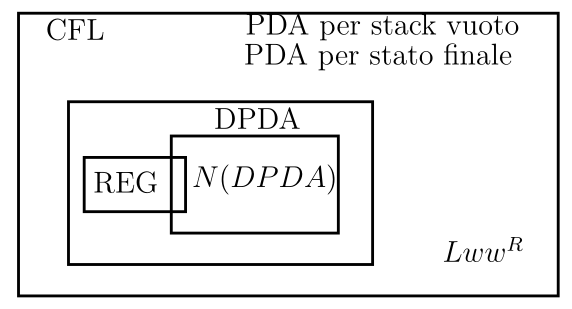
\includegraphics{2025-01-16_15-07.png}
		% \psscalebox{1.0 1.0} % Change this value to rescale the drawing.
		% {
		% 	\begin{pspicture}(0,-2.0)(7.6,2.0)
		% 		\psframe[linecolor=black, linewidth=0.04, dimen=outer](7.6,2.0)(0.0,-2.0)
		% 		\psframe[linecolor=black, linewidth=0.04, dimen=outer](5.0,0.76)(0.7,-1.56)
		% 		\psframe[linecolor=black, linewidth=0.04, dimen=outer](2.38,-0.02)(0.92,-0.82)
		% 		\rput[bl](0.4,1.6){CFL}
		% 		\rput[bl](1.066,-0.54){REG}
		% 		\rput[bl](2.76,0.36){DPDA}
		% 		\rput[bl](3.18,1.18){PDA per stato finale}
		% 		\rput[bl](3.2,1.6){PDA per stack vuoto}
		% 		\rput[bl](5.96,-1.5){$Lww^R$}
		% 		\psframe[linecolor=black, linewidth=0.04, dimen=outer](4.52,0.28)(2.14,-1.12)
		% 		\rput[bl](2.45,-0.56){$N(DPDA)$}
		% 	\end{pspicture}
		% }

	\end{center}
	SI ha che $L_{wcw^R}$ gode della proprietà di prefisso:
	$$y=wcw^R\in L\,\, Se\,\,x\neq y,\mbox{ prefisso di } y,x\not\in L$$
	tornando alle grammatiche si hanno ora due teoremi:
	\begin{theorem}
		se $L=N(P)$ per un DPDA P, allora L ha una CFG non ambigua
	\end{theorem}
	\begin{theorem}
		se $L=L(P)$ per un DPDA P, allora L ha una CFG non ambigua
	\end{theorem}
	dimostriamo il secondo:
	\begin{proof}
		$L=L(P)$ per un DPDA P, costruiamo $L^{'}=L$, quindi $L^{'}$ ha la proprietà di prefisso. Esiste quindi un DPDA $P^{'}$ tale che $L^{'}N(P)$, esiste quindi per il teorema sopra una CFG $G^{'}$ tale che $L(G^{'})=L^{'}$ che non è ambigua.\\
		Costruiamo $G$ per $L$ con le stesse produzioni di $G^{'}$ più $\$\to\varepsilon$, applicata solo all'ultimo passo.
	\end{proof}
	Vogliamo scoprire se è vero il viceversa: per ogni L che ha una CFG non ambigua è vero che L è
	accettato da un DPDA? No, mostriamo infatti un controesempio:\\
$S\to 0S0|1S1|\varepsilon$ produce $L_{ww^R}$ che non è accettato da alcun PDA

	\begin{Exercise}
		costruire un PDA per $L=\{0^n  n| n\geq 1\}$:
		CONTROLLARE LINGUAGGIO
		\begin{center}
			\begin{tikzpicture}[shorten >=1pt,node distance=3cm,on grid,auto]
				\node[state, initial] (q_0) {$q_0$};
				\node[state] (q_1) [right=of q_0] {$q_1$};
				\node[state, accepting] (q_2) [right =of q_1] {$q_2$} ;
				\path[->]
				(q_0) edge [loop above] node [align=center] {$0,0/00$\\$0,z_0/0z_0$} ()
				edge node [align=center] {$1,0/\varepsilon$} (q_1)
				(q_1) edge node {$\varepsilon,z_0/\varepsilon$} (q_2)
				edge [loop above] node [align=center] {$1,0/\varepsilon$} ();
			\end{tikzpicture}
		\end{center}
		Osserviamo che questo è un DPDA e L è accettato sia per stato finale che per stack vuoto.
		Osserviamo anche che L ha la proprietà di prefisso:
		$$y=0^n1^n\in L,x\neq y$$
		e $x$ è prefissa di y e quindi x ha un numero di 0 diverso da quelli di 1 e quindi $x\not\in L$
	\end{Exercise}

	\begin{Exercise}
		costruire un PDA per $L=\{0^n  n|\,n\geq 0\}$:
		\begin{center}
			\begin{tikzpicture}[shorten >=1pt,node distance=3cm,on grid,auto]
				\node[state, initial] (q_0) {$q_0$};
				\node[state] (q_1) [right=of q_0] {$q_1$};
				\node[state, accepting] (q_2) [right =of q_1] {$q_2$} ;
				\path[->]
				(q_0) edge [loop above] node [align=center] {$0,0/00$\\$0,z_0/0z_0$} ()
				edge node [align=center] {$1,0/\varepsilon$} (q_1)
				edge [bend left = 25] node {$\varepsilon,z_0/\varepsilon$} (q_2)
				(q_1) edge node {$\varepsilon,z_0/\varepsilon$} (q_2)
				edge [loop below] node [align=center] {$1,0/\varepsilon$} ();
			\end{tikzpicture}
		\end{center}
		Ora la stringa vuota appartiene al linguaggio. Il linguaggio non ha la proprietà del prefisso. Si può dimostrare che non esiste un DPDA per L.
	\end{Exercise}
	\begin{Exercise}
		considero il linguaggio generato da $B\to (BB)|(B)|()$.\\
		Il linguaggio ha la proprietà di prefisso perché (BB). Se fosse B -> BB allora non lo avrebbe, perché potremmo costruire le stringhe () e ()().
		\\Abbiamo quindi il DPDA per stato finale:
		\begin{center}
			\begin{tikzpicture}[shorten >=1pt,node distance=3cm,on grid,auto]
				\node[state, initial] (q_0) {$q_0$};
				\node[state] (q_1) [right=of q_0] {$q_1$};
				\node[state, accepting] (q_2) [right =of q_1] {$q_2$} ;
				\path[->]
				(q_0) edge [loop above] node [align=center] {$(,z_0/(z_0$\\$(,(/(($} ()
				edge [bend left = 25] node [align=center] {$),(/\varepsilon$} (q_1)

				(q_1) edge node {$\varepsilon,z_0/\varepsilon$} (q_2)
				edge [bend left = 25] node {$(,(/(($} (q_0)
				edge [loop above] node [align=center] {$),(/\varepsilon$} ();
			\end{tikzpicture}
		\end{center}
		volendo accettare solo per stack vuoto:
		\begin{center}
			\begin{tikzpicture}[shorten >=1pt,node distance=3cm,on grid,auto]
				\node[state, initial] (q_0) {$q_0$};
				\node[state] (q_1) [right=of q_0] {$q_1$};
				\path[->]
				(q_0) edge [loop above] node [align=center] {$(,z_0/(z_0$\\$(,(/(($} ()
				edge [bend left = 25] node [align=center] {$),(/\varepsilon$} (q_1)

				(q_1) edge [bend left = 25] node {$(,(/(($} (q_0)
				edge [loop above] node [align=center] {$),(/\varepsilon$ \\ $\varepsilon,z_0/\varepsilon$} ();
			\end{tikzpicture}
		\end{center}
	\end{Exercise}
	\begin{Exercise}
		Si ha $B\to BB|(B)|()$. La stringa vuota non appartiene al linguaggio ma L non ha la proprietà del prefisso (come abbiamo
		mostrato nell'esercizio precedente). Possiamo quindi realizzare solo un DPDA per stato finale:
		\begin{center}
			\begin{tikzpicture}[shorten >=1pt,node distance=3cm,on grid,auto]
				\node[state, initial] (q_0) {$q_0$};
				\node[state] (q_1) [right=of q_0] {$q_1$};
				\node[state] (q_2) [right =of q_1] {$q_2$};
				\node[state,accepting] (q_3) [below right =of q_1] {$q_3$};
				\path[->]
				(q_0) edge node [align=center] {$(,z_0/(z_0$} (q_1)

				(q_1) edge [bend left = 25] node {$),(/\varepsilon$} (q_2)
				edge [loop above] node [align=center] {$(,(/(($} ()
				(q_2) edge [bend left = 25] node {$(,(/(($} (q_1)
				edge [loop above] node [align=center] {$),(/\varepsilon$} ()
				edge node {$\varepsilon,z_0/z_0$} (q_3)
				(q_3) edge node {$(,z_0/(z_0$} (q_1)  ;
			\end{tikzpicture}
		\end{center}
	\end{Exercise}
	\begin{Exercise}
		Si ha $B\to BB|(B)|\varepsilon$ ho un DPDA per stato finale perché L non ha la proprietà del prefisso:
		\begin{center}
			\begin{tikzpicture}[shorten >=1pt,node distance=3cm,on grid,auto]
				\node[state, initial,accepting] (q_0) {$q_0$};
				\node[state] (q_1) [right=of q_0] {$q_1$};
				\node[state] (q_2) [right =of q_1] {$q_2$};

				\path[->]
				(q_0) edge node [align=center] {$(,z_0/(z_0$} (q_1)

				(q_1) edge [bend left = 25] node {$),(/\varepsilon$} (q_2)
				edge [loop above] node [align=center] {$(,(/(($} ()
				(q_2) edge [bend left = 25] node {$(,(/(($} (q_1)
				edge [loop above] node [align=center] {$),(/\varepsilon$} ()
				edge [bend left = 65] node {$\varepsilon,z_0/z_0$} (q_0);
			\end{tikzpicture}
		\end{center}
	\end{Exercise}
	\begin{Exercise}
		sia $L=\{q\in\{a,b\}^*| numero\,\,uguale\,\,di\,\,a\,\,e\,\,b\}$ DPDA per stato finale (L non ha la proprietà di prefisso):
		\begin{center}
			\begin{tikzpicture}[shorten >=1pt,node distance=3cm,on grid,auto]
				\node[state, initial,accepting] (q_0) {$q_0$};
				\node[state] (q_1) [right=of q_0] {$q_1$};
				\path[->]
				(q_0) edge [bend left=25] node [align=center] {$b,z_0/bz_0$\\$a,z_0/az_0$} (q_1)

				(q_1) edge [bend left = 25] node {$\varepsilon,z_0/z_0$} (q_0)
				edge [loop above] node [align=center] {$a,a/aa$\\$b,b/bb$\\$a,b/\varepsilon$ \\$b,a/\varepsilon$} ()
				;
			\end{tikzpicture}
		\end{center}
	\end{Exercise}
	\newpage
	\begin{Exercise}
		sia dato il CFL $L=\{a^ncb^n|n\geq 0\}$\\
		è generato da :
		$$G=(\{S\},\{a,b,c\},P,S)$$
		$$S\to aSb|c$$
		si ha il seguente automa non deterministico:
		\begin{center}
			\begin{tikzpicture}[shorten >=1pt,node distance=3cm,on grid,auto]
				\node[state, initial,accepting] (q_0) {$q_0$};
				\path[->]
				(q_0) edge [loop above] node [align=center] {$\varepsilon,S/aSb$\\$\varepsilon,S/c$\\$a,a/\varepsilon$\\$b,b/\varepsilon$\\$c,c/\varepsilon$} ();
			\end{tikzpicture}
		\end{center}
		con:
		$$\delta(q,\varepsilon,S)=\{(q,aSb),(q,c)\}$$
		$$\delta(q,a,a)=\{(q,\varepsilon)\}$$
		$$\delta(q,b,b)=\{(q,\varepsilon)\}$$
		$$\delta(q,c,c)=\{(q,\varepsilon)\}$$
		mostro la derivazione per n=3, aaacbbb e il comportamento dell'automa:
		$$(q,aaacbbb,S)\vdash(q,aaacbbb,aSb)\vdash(q,aacbb,Sb)\vdash(q,aacbb,aSb)$$
		$$\vdash(q,acbbb,Sbb)\vdash(q,acbbb,aSbbb)\vdash(q,cbbb,Sbbbb)\vdash(q,cbbb,cbbb)$$
		$$\vdash(q,bbb,bbb)\vdash(q,bb,bb)\vdash(q,b,b)\vdash(q,\varepsilon,\varepsilon)\to \,\, accetta$$
		si ha che vale la proprietà del prefisso e si ha il seguente DPDA:
		\begin{center}
			\begin{tikzpicture}[shorten >=1pt,node distance=3cm,on grid,auto]
				\node[state, initial,accepting] (q_0) {$q_0$};
				\node[state] (q_1) [right=of q_0] {$q_1$};
				\node[state] (q_2) [right =of q_1] {$q_2$};
				\path[->]
				(q_0) edge node [align=center] {$c,z_0/cz_0$\\$c,a/a$} (q_1)
				edge [loop above] node [align=center] {$a,z_0/az_0$\\$a,a/aa$} ()
				(q_1) edge  node {$\varepsilon,z_0/z_0$} (q_2)
				edge [loop above] node [align=center] {$b,a/\varepsilon$} ();
			\end{tikzpicture}
		\end{center}
	\end{Exercise}
	\begin{Exercise}
		realizzare il pda per $L=\{a^nb^mcd^mef^n|n,m\geq 0\}$;
		si ha quindi:
		$$a^ncef^n\,\,n>0$$
		$$b^mcd^me\,\,m>0$$
		$$a^nb^mcd^mef^n\,\,n,m> 0$$
		$$ce\,\,n=0=m$$
		\begin{center}
			\begin{tikzpicture}[shorten >=1pt,node distance=3cm,on grid,auto]
				\node[state, initial] (q_0) {$q_0$};
				\node[state] (q_1) [above right=of q_0] {$\mbox{ }$};
				\node[state] (q_2) [right =of q_0] {$\mbox{ }$};
				\node[state] (q_3) [below right =of q_0] {$\mbox{ }$};
				\node[state] (q_4) [ right =of q_1] {$\mbox{ }$};
				\node[state] (q_5) [above =of q_1] {$\mbox{ }$};
				\node[state] (q_6) [right =of q_2] {$\mbox{ }$};
				\node[state,accepting] (q_7) [right =of q_6] {$\mbox{ }$};
				\node[state] (q_8) [right =of q_5] {$\mbox{ }$};
				\node[state] (q_9) [right =of q_8] {$\mbox{ }$};
				\node[state] (q_a) [right =of q_4] {$\mbox{ }$};

				\path[->]
				(q_0) edge node [align=center] {$a,z_0/az_0$} (q_1)
				(q_0) edge node [align=center] {$b,z_0/bz_0$} (q_2)
				(q_0) edge node [left] {$c,z_0/cz_0$} (q_3)
				(q_2) edge node [align=center] {$c,b/b$} (q_6)
				edge [loop below] node [align=center] {$b,b/bb$} ()
				(q_6) edge node [align=center] {$\varepsilon,z_0/z_0$} (q_7)
				edge [loop below] node [align=center] {$d,b/\varepsilon$} ()

				(q_3) edge [bend right =65] node [align=center] {$\varepsilon,z_0/z_0$} (q_7)
				(q_1) edge node [align=center] {$b,a/ba$} (q_5)
				edge node [align=center] {$c,a/ca$} (q_4)
				edge [loop left] node [align=center] {$a,a/aa$} ()
				(q_5) edge node [align=center] {$c,b/cb$} (q_8)
				edge [loop above] node [align=center] {$b,b/bb$} ()
				(q_8) edge node [align=center] {$e,a/a$} (q_9)
				edge [loop above] node [align=center] {$d,b/\varepsilon$} ()
				(q_9) edge [bend left =95] node [align=center] {$\varepsilon,z_0/z_0$} (q_7)
				edge [loop above] node [align=center] {$f,a/\varepsilon$} ()
				(q_4) edge node [align=center] {$e,a/a$} (q_a)
				(q_a) edge node [align=center] {$\varepsilon,z_0/z_0$} (q_7)
				edge [loop right] node [align=center] {$f,a/\varepsilon$} ()
				;


			\end{tikzpicture}
		\end{center}
	\end{Exercise}

	\newpage
\section{Soluzioni degli esercizi}
\label{sec:soluzioni-cfg}
\shipoutAnswer

%%% Local Variables:
%%% mode: LaTeX
%%% TeX-master: ../libro-linguaggi
%%% End:

